%   SETUP%
\documentclass[a4paper,11pt,oneside,titlepage]{book}
\usepackage[T1]{fontenc}		% Codifica dei font; T1 codifica di output dell'italiano e di lingue occidentali
\usepackage[utf8]{inputenc}		% Codifica degli input; abilita l'utilizzo di caratteri accentati
\usepackage[english]{babel}		% Set the languages; the last one is the main language
\usepackage{geometry}			% Allow to change the margin
\usepackage{setspace}			% Allow to change the interline with \begin{onehalfspaceng} ecc.
\usepackage{fancyhdr}			% Fancy style for page layout
\usepackage{afterpage} 			% Allow to load blank pages with the command '\afterpage{\null\thispagestyle{empty}\clearpage}' 
\usepackage{hyperref}			% Crea collegamenti ipertestuali rendendo cliccabili i riferimenti
\usepackage{url}
\usepackage{amsthm}
\usepackage{amssymb}
\usepackage{color}			% Allow to use colors
\usepackage{xcolor}			% manage colors
\usepackage{enumerate}			% Numbered lists
\usepackage{enumitem}			% Allow to manage the style of the list
\usepackage{graphicx}			% Images
\usepackage{epstopdf}			% allows to convert eps images to pdf for use with pdflatex
\usepackage{pstool}			% Allows to use psfrag with pdflatex (no latex compiler needed)
\usepackage{psfrag}
% \usepackage[normal]{subfigure}		% manage subfigures
% \usepackage{subfig}		% manage subfigures
\usepackage{array}			% Tables
\usepackage{tabularx}			% allow to set the width of the whole table
\usepackage[bottom]{footmisc}		% To attach footnote at the end of the page
\usepackage{booktabs}			% is a must for professional-looking layout
\usepackage{longtable}			% is very popular for multi-page tables
\usepackage{caption}			% Captions
\usepackage{float}			% Manage float objects (image, table, ecc.)
\usepackage{rotating}			% permette di ruotare immagini, tabelle, ecc. di 90° o di 270°
\usepackage{rotfloat}			% costruisce un ponte tra i pacchetti float e rotating
\usepackage{amsmath} 			% Equations
\usepackage{amssymb}			% Mathematical Symbols
\usepackage{cancel}                     % Simplification Cancellation
\usepackage{mleftright}
\usepackage{algorithm}              % Algorithm
\usepackage{algpseudocode}
\usepackage{listings}                   % Codes
\definecolor{lstgreen}{rgb}{0,0.6,0}
\definecolor{lstgray}{rgb}{0.5,0.5,0.5}
\definecolor{lstmauve}{rgb}{0.58,0,0.82}
\lstset{ %
  backgroundcolor=\color{white},   % choose the background color
  basicstyle=\footnotesize,        % size of fonts used for the code
  breaklines=true,                 % automatic line breaking only at whitespace
  captionpos=b,                    % sets the caption-position to bottom
  commentstyle=\color{lstgreen},    % comment style
  escapeinside={\%*}{*)},          % if you want to add LaTeX within your code
  keywordstyle=\color{blue},       % keyword style
  stringstyle=\color{lstmauve},     % string literal style
}
%\usepackage{vector}  			% Allows "\bvec{}" and "\buvec{}" for "blackboard" style bold vectors in maths
\usepackage[swapnames,norules,nouppercase]{frontespizio}
\usepackage[intoc]{nomencl}
\usepackage[acronym,toc,nomain,nopostdot,nonumberlist]{glossaries}
\usepackage[square, numbers, comma, sort&compress]{natbib}
\usepackage{verbatim}                   % Needed for the "comment" environment to make LaTeX comments
\usepackage{wrapfig}                 % Per inserire le figure contornate da testo
\usepackage{blindtext}
\usepackage{graphicx}
\usepackage{subcaption}
\geometry{a4paper,top=2.5cm,bottom=2.5cm,left=2cm,right=2cm,heightrounded,bindingoffset=5mm,headheight=13.6pt}
% -------------------------------------- Line-spacing --------------------------------------- %
\linespread{1.2} 
%\linespread{1.5} 
%\linespread{2} 
%\raggedbottom % disattiva lo 'stiracchiamento' del testo; va a favore di spazio bianco a fondo pagina
% ---------------------------------------- Numeration --------------------------------------- %
%\setcounter{secnumdepth}{3} % set the enumeration of the sections
%\setcounter{tocdepth}{3}    % set the enumeration of the sections in the table of contents
%--------------------------------------- Page layout -----------------------------------------%
%\pagestyle{fancy}                       % definisce lo stile di pagina aprendo la strada al pacchetto fancyhdr
%\renewcommand{\chaptermark}[1]{\markright{\chaptername\ \thechapter.\ #1}{}}    % ridefinisce la macro \rightmark per i capitoli
%\renewcommand{\sectionmark}[1]{\markright{\sectionname\ \thesection.\ #1}}      % ridefinisce la macro \rightmark per le sezioni
%\renewcommand{\sectionmark}[1]{\markright{\thesection.\ #1}}
%\lhead{Giacomo Della Posta}             % in alto a sinistra
%\chead{}                                % in alto al centro
%\rhead{\slshape \rightmark}             % in alto a destra (\rightmark contiene ...)
%\lfoot{Giacomo Della Posta}             % in basso a sinistra
%\cfoot{\thepage}                        % in basso al centro (\thepage per mettere il numero di pagina)
%\rfoot{}                                % in basso a destra
%\renewcommand{\headrulewidth}{0.4pt}    % spessore della linea di separazione in alto (0 per eliminare la linea)
%\renewcommand{\footrulewidth}{0.4pt}    % spessore della linea di separazione in basso (0 per eliminare la linea)
\fancypagestyle{plain}{%                                        % modifica dello stile predefinito plain
                        \fancyhf{}                              % cancella tutti i campi di  intestazione e pie di pagina
                        \fancyfoot[R]{\thepage}                 % mette al centro il numero di pagina
                        \renewcommand{\headrulewidth}{0pt}      % spessore della linea di separazione in alto (0 per eliminare la linea)
                        \renewcommand{\footrulewidth}{0.4pt}    % spessore della linea di separazione in basso (0 per eliminare la linea)
                        }                                       % modifica dello stile predefinito plain
\captionsetup{font=small,labelfont=bf,textfont=normalfont,tableposition=bottom,figureposition=bottom}
%\captionsetup{font=small,labelfont=bf,textfont=bf,tableposition=bottom,figureposition=bottom}
% ---------------------------------------- Itemize ------------------------------------------ %
%\setlist[itemize]{noitemsep, topsep=0pt} %Se non vuoi i pallini degli elenchi vuoti, allora commenta queste linee      
%\renewcommand{\labelitemi}{$\circ$}	% items i with empty bullets
%\renewcommand{\labelitemii}{$\bullet$}	% items ii with black bullets
\hypersetup{colorlinks=true, linkcolor=black, citecolor=black, filecolor=black, urlcolor=black}
\definecolor{red-univaq}{RGB}{130,36,51} % example \definecolor{name}{model}{color-spec}
\definecolor{univaq}{RGB}{242,195,80} % example \definecolor{name}{model}{color-spec}
\makenomenclature % Generate the nomenclature
\makeglossaries % Generate the glossary
%\lstset{language=[90]Fortran,
%        inputpath=/home/luca/PhD/Thesis/Code,
%        basicstyle=\small\ttfamily, 
%        xleftmargin=0cm,
%        fontadjust=true,
%        keepspaces=true,
%        basewidth=0.5em,
%        breakatwhitespace=false,           % sets if automatic breaks should only happen at whitespace
%        breaklines=false,                  % sets automatic line breaking
%        captionpos=b,                     % b=bottom
%        backgroundcolor=\color{white},
%        identifierstyle=\color{black},
\bibliographystyle{abbrv} % abbrv --> [1], [2], ecc.
%\bibliographystyle{unsrtnat} 
% ---------------------------------------- Dedication ------------------------------------------ %
\newenvironment{dedication}
{
  \phantom{.}
  \vspace{13cm}
  \begin{quote} \begin{flushright}}
{\end{flushright} \end{quote}}
\usepackage{calligra}

\begin{document}

%   FRONT MATTER                                            %
\frontmatter 	   % Begin Roman style (i, ii, iii, iv...) page numbering
\pagestyle{empty}  % No headers or footers for the following pages

%   TITLE PAGE]


\begin{frontespizio}
% Remember: After editing this file, delete the cache and recompile
%---------------------Definizione font---------------------%
\Preambolo{\renewcommand{\fronttitlefont}{\fontsize{24}{24}\bfseries}}
%----------------------------------------------------------%
	% \frontinstitutionfont 	Neretto, 14/17 
	% \frontdivisionfont 		Tondo, 12/16 
	% \frontpretitlefont 		Maiuscoletto, 10/12
	% \fronttitlefont 		Neretto, 17/21 
	% \frontsubtitlefont 		Tondo, 12/14
	% \frontfixednamesfont 		Tondo, 12/14 
	% \frontnamesfont 		Neretto, 12/14 
	% \frontsmallfont 		Neretto, 9/11 
	% \frontfootfont	 	Neretto, 12/14 

	% \bfseries	Grassetto
	% \itshape	Corsivo
	% \scshape	Maiuscoletto
%----------------------------------------------------------%
\Margini{4cm}{3cm}{3cm}{3cm} % Margini sinistro, in basso, destro e in alto
\Logo[4cm]{figures/logo/UnivAQ_logoA.eps}
%\Universita{L'Aquila}
\Istituzione{Dipartimento di Ingegneria e Scienze dell'Informazione e Matematica}
% \Istituzione{Department of Information Engineering, Computer Science and Mathematics}
% \Divisione{Department of Information Engineering, Computer Science and Mathematics}	% ENG
% \Divisione{Tesi di Laurea Magistrale in Ingegneria Matematica}		% ITA
    \Divisione{Master’s Thesis in Mathematical Engineering}
%\Dipartimento{Dipartimento di Ingegneria e Scienze dell'Informazione e Matematica}
%\Corso[Master Degree]{Ingegneria delle Telecomunicazioni}
\Scuola{}
\Titoletto{}

\Titolo{Experiments with Dataless Neural Networks to solve the Maximum Independent Set Problem}
%\Sottotitolo{}

\Punteggiatura{} % Modifica la punteggiatura dopo 'Candidato', 'Realatore' ecc. (vuoto per togliere)
\NCandidato{Candidate} % Sostituisce 'Candidato' con '...'
\Preambolo{\renewcommand{\frontsmallfont}[1]{\small}}
\Candidato{Kyrylo Vdovin}

%\NRelatore{Thesis Advisor}{Relatori}
\NRelatore{Supervisor}{Relatori}
\Relatore{Prof. Fabrizio Rossi}
%\NCorrelatore{Thesis Co-Advisor}{Relatori}
\NCorrelatore{Co-Supervisor}{Relatori}
\Correlatore{Dr. Andrea Manno}
%\Rientro{1cm} % Rientro di Relatore e Candidato

\Piede{A.Y. 2021-2022}
\end{frontespizio}

\IfFileExists{\jobname-frn.pdf}{}{%
\immediate\write18{pdflatex \jobname-frn}} 
\clearpage

%   TOC - LOF - LOT
\begin{singlespace}
 \tableofcontents 	
 \addcontentsline{toc}{chapter}{\listfigurename}
 \listoffigures
 \addcontentsline{toc}{chapter}{\listtablename}
 \listoftables
 \clearpage
 
% \renewcommand{\lstlistlistingname}{List of Code}
% \addcontentsline{toc}{chapter}{\lstlistlistingname} 
% \lstlistoflistings

%   NOMENCLATURE AND ACRONYMS
%  \printnomenclature
%  \printglossaries
\end{singlespace}

%   ABSTRACT
% \afterpage{\null\thispagestyle{empty}\clearpage} % Blank page
\thispagestyle{plain}			% Supress header 
\setlength{\parskip}{0pt plus 1.0pt}
\section*{Abstract}

This thesis considers the problem of search the maximum independent set in an undirected graph. An independent set is a group of vertices where no two vertices are neighboring. A lot of real life problems in biochemistry,  converge to max independent search and thus creating efficient algorithm is a challenging and multipurpose task. To date, there is no effective algorithm for locating the most independent sets. In contrast to the general greedy methods for MIS, evolutionary algorithms, supervised learning neural networks, we want to provide a dataless neural network algorithm based only on the graph structure and that does not require training data. We also provide algorithms for large graphs reducton based on communities detection and a few preprocessing and postprocessing tecnhics for reducing graph cardinality and improving result of the neural network. Our model performs on average with 90 \% accuracy comparing to existing state-of-art methods but generates sub-optimal result exponentially faster than other solvers so it can be used for getting sub-optimal solutions on large graphs.

\vfill

\thispagestyle{empty}
\mbox{}

\clearpage

\section*{Acknowledgements}
I wish to thank Professors Fabrizio Rossi and Andrea Manno for their guidance throughout this project. 
I would like to thank my parents and my sister for their love and support. Finally, thanks to my friends for proofreading and general encouragement. 

%   MAIN MATTER
\mainmatter	  % Begin normal, numeric (1,2,3...) page numbering
\clearpage
% ------ set page style fancy with the follow 
\pagestyle{fancy} 
\renewcommand{\chaptermark}[1]{\markright{\chaptername\ \thechapter.\ #1}{}}
\renewcommand{\sectionmark}[1]{\markright{\thesection.\ #1}}
\lhead{} 
\chead{}                   
\rhead{\slshape \rightmark} 
\lfoot{Kyrylo Vdovin}
\cfoot{} 
\rfoot{\thepage}          
\renewcommand{\headrulewidth}{0.4pt} 
\renewcommand{\footrulewidth}{0.4pt}

% Shortcuts
\newcommand{\graphG}{$G=(V,E)$ }

%   CHAPTERS
\chapter{Maximum independent set problem}
\section{Purpose of study}
Optimization has been expanding in all directions at an astonishing rate during
the last decades. New algorithmic and theoretical techniques have been developed,
the diffusion into other disciplines has proceeded at a rapid pace, and our knowledge
of all aspects of the field has grown even more profound. At the same time,
one of the most striking trends in optimization is the constantly increasing emphasis on the interdisciplinary nature of the field. Optimization today is
basic research
tool in all areas of engineering, medicine and the sciences. The decision making tools
based on optimization procedures are successfully applied in a wide range of practical
problems arising in virtually any sphere of human activities, including biomedicine,
energy management, aerospace research, telecommunications and finance.

Practical applications of the considered optimization problems are abundant.
They appear in information retrieval, signal transmission analysis, classification
theory, economics, scheduling, experimental design, and computer vision. Among the known problems 
that come down to finding an independent set are the following: 
matching molecular structure \cite{molecular_matching}, 
macromolecular docking \cite{molecular_docking},
integration of genome mapping data \cite{genome_mapping}, 
comparative modeling of protein structure\cite{modeling_protein_structure}, covering location using clique partition \cite{butenko_applications} etc.

Considering the theoretical significance and practical relevance of the MCP, a lot of time and attention has been put into developing different solution methods. On the one hand, the generic branch-and-bound (B\&B) framework has served as the foundation for several useful accurate approaches. These techniques offer the potential benefit of ensuring that the answer found is the best one possible. However, due to the MCP's intrinsic computational complexity, accurate techniques sometimes only work for small issues and can be computationally expensive in general. On the other hand, several heuristic and metaheuristic algorithms have been developed with the aim of delivering sub-optimal solutions to huge problems that can't be solved optimally in a reasonable amount of time.

A lot of real life problems use graph theory and converge to maximum clique problem. Finding the maximum clique $MC$ in the graph $G$ is $NP$-hard problem and is the same as finding maximum independent set $MIS$ on the complementary graph $G'$. 

\section{Problem definition}
Given an undirected graph \graphG where $V$ - finite set of vertices and $E$ - finite set of edges.

\newtheorem{definition}{Definition}[section]
\begin{definition} [Complement graph]
Complement graph $G'=(V,E')$ is a graph s.t. for $\forall e\in E' \iff e\notin E$ 
\end{definition}
\begin{definition} [Clique]
Clique $C$ in an undirected graph \graphG is a subset of vertices $C\subseteq V$ such that every two distinct vertices are adjacent. This is equivalent to the condition that the induced subgraph of G induced by C is a complete graph.
\end{definition}
\begin{definition} [Maximal clique]
Maximal clique $MaxC$ is a clique that cannot be extended by including one more adjacent vertex, that is, a clique which does not exist exclusively within the vertex set of a larger clique.
\end{definition}
\begin{definition} [Maximum clique]
Maximum clique $MC$ of a graph \graphG is a clique, such that there is no clique with more vertices. Moreover, the clique number $\omega(G)$ of a graph $G$ is the number of vertices in a maximum clique in $G$.
\end{definition}
\begin{definition}[Independent set]
Independent set in graph \graphG is a set of vertices $S \subseteq V$ such that no vertices in $S$ are adjacent to each other.
\end{definition}

For a subset $U$ of vertices $V$ of graph \graphG $U \subseteq V$, $G[U] = (U,E[U])$ is used to represent the subgraph \textbf{induced} by $U$, s.t. edges of $U$ is a set $E[U] = \{(u,v)\in E | u,v\in U\}$

\begin{figure}[h]
    \centering
    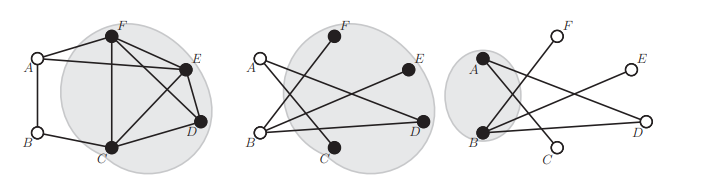
\includegraphics{figures/graph_clique_IS_dependencies.png}
    \caption{An illustration of the relation between maximum clique, maximum independent set and minimum vertex cover. Given the initial graph $G$ with $V = \{A, B, C,D, E, F\}$(left) and its complementary graph $G$ (middle/right), the set of vertices $\{C,D, E, F\}$ is a maximum clique of $G$ and an maximum independent set of $G$ while ${A, B} = V \ {C,D, E, F}$ is a minimum vertex cover of $G$}
    \label{fig:graph_clique_IS_dependencies}
\end{figure}

\begin{definition}[Maximum independent set problem]
The Maximum Independent Set \textit{MIS} problem in graph theory is the task of finding
the largest independent set in a graph.
\end{definition}

There are many research on the MIS formulation. These investigations hold a great deal of interest since they have the potential to deepen our understanding of the issue at hand and yield novel theoretical and applied findings.
The following binary problem gives the simplest formulation:
\begin{subequations} \label{mis_binary_formulation_1}
\begin{equation} 
    \text{maximize} \sum_{i=1}^n x_i
\end{equation}
\begin{equation}
    \text{subject to } x_i+x_j \leq 1, \forall \{i,j\}\in E
\end{equation}
\begin{equation}
    x_i \in \{0,1\}, i = 1,...,n
\end{equation}
\end{subequations}

An alternative formulation of this problem is the following \textit{clique formulation}:
\begin{subequations}\label{clique_binary_formulation_1}
\begin{equation}
    \text{maximize} \sum_{i=1}^n x_i
\end{equation}
\begin{equation} \label{clique_binary_formulation_2}
    \text{subject to } x_i \leq 1, \forall S \in C \equiv \text{\{maximal cliques of $G$\}}
\end{equation}
\begin{equation}
    x_i \in \{0,1\}, i = 1,...,n
\end{equation}
\end{subequations}

The advantage of formulation \ref{clique_binary_formulation_1} over \ref{mis_binary_formulation_1} is a smaller gap between the optimal
values of \ref{clique_binary_formulation_1} and its linear relaxation, however
 finding a good solution to \ref{clique_binary_formulation_1} is challenging since the number of restrictions in \ref{clique_binary_formulation_2} is exponential.

 Here we mention one more integer programming formulation. Let $A_G$ be the
adjacency matrix of a graph \graphG, and let $J$ denote the $nxn$ identity matrix. The
maximum independent set problem is equivalent to the global quadratic zero-one problem
\begin{subequations} \label{mis_matrix_furmulation}
\begin{equation}
    \max f(x) = x^TAx   
\end{equation}
subject to 
\begin{equation}
    x_i \in \{0,1\}, i = 1,...,n
\end{equation}
\end{subequations}
where $A = J - A_G$. If $x^*$ is a solution to \ref{mis_matrix_furmulation}, then the set $\mathcal{I}$ defined by $\mathcal{I}=\{i\in V:{x_i}^*=1\}$ is the MIS of $G$ with $|\mathcal{I}|=f(x^*)$.

The independent set problem and the clique problem are complementary: a clique in \graphG is an independent set in the complement graph of $G$ and vice versa. Therefore, many computational results may be applied equally well to either problem. For example, the results related to the clique problem have the following corollaries:

\begin{itemize}
    \item The independent set decision problem is $NP$-complete, and hence it is not believed that there is an efficient algorithm for solving it.
    \item The maximum independent set problem is $NP$-hard and it is also hard to approximate.
\end{itemize}

Despite the close relationship between maximum cliques and maximum independent sets in arbitrary graphs, the independent set and clique problems may be very different when restricted to special classes of graphs. For instance, for sparse graphs (graphs in which the number of edges is at most a constant times the number of vertices in any subgraph), the maximum clique has bounded size and may be found exactly in linear time.

There is currently no known efficient algorithm to find maximum independent sets, however there are powerful heuristic algorithms to solve this problem like ReduMIS \cite{redumis}, IBM CPLEX LP-solver \cite{CPLEX}, branch-reduce algorithms and others. The most recent state-of-art solver ReduMIS uses iterative implementation of a series of graph reduction techniques and evolutionary algorithm. CPLEX uses plain integer linear programming solving to obtain the solution. Despite these algorithms return quite accurate results they have large disadvantage - they are very time consuming and not appropriate for large graphs regarding memory consumption. 
The main idea of improvement is to use algorithm that can obtain solution in more parallelized way using neural networks.

\section{Heuristics for MIS problem}
Even on graphs with several hundred vertices, exact approaches become impractical (too slow) despite providing the best solution. Because of this such approaches cannot be used to solve the maximum independent set problem on very large graphs, thus heuristic solutions are the ones that can be used.
Perhaps the most straightforward heuristics for the maximum independent set problem are sequential greedy heuristics, which repeatedly add a vertex to an intermediate independent set ("Best in") or remove a vertex from a set of vertices that is not an independent set ("Worst out") based on some criterion, say the degrees of the vertices \cite{j74}, \cite{kr87}.
People occasionally look to nature for effective heuristics because it always seems to have the best answers. New types of optimization algorithms that essentially try to mimic specific natural processes have recently been created and successfully tested.

The design of simulated annealing \cite{kgv83}, neural networks \cite{h82}, and evolutionary computation \cite{h75} methods in the field of optimization were influenced by the natural phenomenal observed in annealing processes, nervous systems, and natural evolution. Other well-liked metaheuristics are tabu search \cite{gl97} and greedy randomized adaptive search procedures, or GRASP \cite{fr95}. These heuristics have been successfully used in various forms to solve numerous significant combinatorial optimization issues, including the maximum independent set problem. Below, we'll quickly go over a few of these heuristics.

\subsection{Greedy randomized algorithm}
An iterative randomized sampling technique called a greedy randomized adaptive search procedure (GRASP) provides a heuristic solution to the current problem with each iteration \cite{fr95} in a subtle way. The final outcome for all intents and purposes is literally the best solution across all GRASP iterations. Each GRASP iteration consists of two phases: the first creates a restricted candidate list (RCL) of solutions using an adaptive randomized greedy function; the second one attempts to find an improvement by using a local search technique. 
The so-called path relinking \cite{glm00} , a recent addition to GRASP, has been proposed to improve the performance of the heuristic by connecting good quality solutions with a path of intermediate feasible points. It seems that many of these possible places offer solutions of higher quality than the ones picked as the path's endpoints. For difficult problems with the maximal independent set or graph coloring, the GRASP approach with path relinking can be used.

The success of machine learning solutions for reasoning about discrete structures has brought attention to its adoption within combinatorial optimization algorithms. These approaches usually rely on supervised learning by leveraging datasets of the combinatorial structures of interest drawn from some distribution of problem instances. Reinforcement learning has also been employed to find such structures. We propose an approach such that no data is necessary for training the networks that produce the solution. The suggested technique is not machine learning in this sense. However, it relies on neural networks and applies backpropagation to a loss function determined by the architecture of the neural network rather than a training dataset. To handle large-scale graphs, we also suggest a general graph reduction method. The reduction, which works with any graph type and/or density, takes advantage of community detection for graph splitting. Also some postprocessing of the neural network result is included to improve the final result.

\subsection{Genetic algorithms}

Natural system evolution processes served as the inspiration for genetic algorithms in optimization. A population of points, also known as individuals or chromosomes, are used for optimization in a genetic algorithm. The chromosomes are represented in the most basic form by binary vectors. Each chromosome has a fitness value, which measures the likelihood that the person designated by that chromosome will live to adulthood in the following generation. Values of the objective function that represents the population's overall fitness are computed using individual fitness values. An optimization technique may be built on the fundamental law of natural selection, which states that population fitness as a whole doesn't decline with time.

The genetic algorithm, in its most basic form, begins with a population selected at random and computes a new population using one of three fundamental mechanisms: reproduction, crossover, or mutation \cite{g89}. According to the likelihood provided by their fitness, the reproduction operator selects the chromosomes employed in the following generation. To create additional offspring from a pair of parents and children, the crossover operator is used. Finally, the mutation operator, with a specified probability, flips the value of each bit in a chromosome.

From the beginning of the 1990s, early attempts were made to use genetic algorithms to solve the maximum independent set and maximum clique problems. Since then, several effective implementations have been documented in the literature \cite{be95}, \cite{h97}, \cite{m02}. The majority of genetic algorithms are simple to parallelize.

\subsection{Simmulated annealing}

In physics, the annealing procedure is used to create a pure lattice structure. It entails heating a solid to melt it, followed by progressively cooling it to a low-energy state to solidify it. This procedure minimizes the free energy of the system. In the simulated annealing approach, where each viable solution represents a state of the fictitious physical system and the objective function represents the energy corresponding to that state, this characteristic of the annealing process is employed for optimization purposes. The following is the fundamental idea of simulated annealing:
Generate an initial feasible solution $x^{(0)}$. On the iteration $k+1$, given a solution $x^{(k)}$, accept it's neighbours $x^{(k+1}$ as the next feasible solution with probability
\begin{equation}
   \begin{cases}
      1, & \text{if} f(x^{k+1}) < f(x^k);\\
      \exp, \frac{f(x^{k+1})-f(x^k)}{t} & \text{otherwise}
    \end{cases}  
\end{equation}
where $f(x)$ is cost function and $t$ is a temperature parameter that changes while the optimization process is carried out. One of the most crucial components of the algorithm is the appropriate selection of the cooling schedule that describes the change in the temperature parameter. In theory, a cooling plan that is logarithmically slow will produce the best result in an exponential amount of time, but in actuality, cooling schedules that are faster will produce results that are acceptable.

Aarts and Korst \cite{ak89} provided a description of simulated annealing for the maximal independent set issue using a penalty function technique in their textbook. They utilized a cost function of the type $f(V') = |V'| - \lambda |E'|$, where $V' \subset V$ is the provided subset of vertices and $E' \subset V' x V'$ is the set of edges in $G(V')$. Aarts and Korst's approach was modified by Homer and Peinado \cite{hp96} using a straightforward cooling schedule, and their results for the maximum clique issue were contrasted with those of various other heuristics. They came to the conclusion that the simulated annealing method outperformed the competing strategies on the examples under consideration after conducting trials on networks with up to 70,000 vertices.

\subsection{Tabu search}

In order to eliminate repeatitions when exploring the space of possible solutions, \textit{tabu} search is a variant of local search algorithms.
Maintaining a set of \textit{tabu} lists with the routes of workable solutions that the algorithm has previously considered allows for the implementation of such a technique. The best legal (not forbidden by the \textit{tabu} method) option in the immediate vicinity of the present solution, even if it is worse than the current solution, is considered the next potential solution.
The MIS and MaxC problems have been successfully solved using various \textit{tabu} algorithms \cite{bp01}, \cite{fhw89}, \cite{ms99}, \cite{ss82}.

\subsection{Continious comninatorial optimization}
Continuous methods to combinatorial optimization issues seem to be very appealing, as was described above. The Motzkin-Straus formulation, which connects the clique number of a graph to a quadratic program, was at the center of recent efforts to construct continuous-based heuristics for the maximum independent set and maximum clique issues.

Recently, semidefinite programming approaches, which are basically continuous, saw their foundation and quick growth. The groundbreaking finding by Goemans and Williamson marked a significant advancement in the development of approximation algorithms and demonstrated the critical role semidefinite programming plays in combinatorial optimization. Burer et al. developed two continuous optimization formulations for the largest independent set issue by taking into account rank-one and rank-two relaxations of the Lov'asz semidefinite program.
They created and put to the test fresh algorithms for locating big independent sets based on these formulations.

\subsection{Neural networks}
Recent years have seen a rise in the use of neural networks as a tool for a variety of complicated issue solving. Artificial intelligence that replicates the activity of organic neurons is known as a neural network. They are made up of nodes, which are made up of layers of artificial neurons coupled together. In response to input data, the nodes can modify their behavior and communicate with one another. Neural networks are able to learn from data and may be applied to categorize, spot patterns in data, and generate predictions. Similar to biological nervous systems, neural networks exhibit tremendous levels of connectivity and huge parallelism.

Machine learning's incorporation into combinatorial optimization algorithms has received interest due to its efficacy in solving discrete structure reasoning problems. These methods often use datasets of the relevant combinatorial structures that are selected from a range of issue occurrences and rely on supervised learning. Such structures have also been discovered via reinforcement learning. 

Although neural networks were first used in the late 1950s, it wasn't until the development of sufficiently sophisticated related methods in the middle of the 1980s that they were extensively used. According to Hopfield and Tank, some neural network models may be utilized to roughly solve a number of challenging combinatorial optimization issues. Neural networks are used nowadays to solve a wide variety of challenging real-world issues like car driving, facial recognition, healthcare, defence.

Since the late 1980s, several researchers have used various neural network variants to tackle the maximal independent set issue. Due to the absence of experimental data, it is challenging to assess the effectiveness of early endeavors.
We shall thus discuss a few of the more recent contributions. For the maximal clique, Grossman took into account a discrete version of the Hopfield model in the year 1996.

Computing studies using this strategy on the DIMACS benchmarks produced excellent results, although they lagged behind other rival approaches like simulated annealing. For the maximum clique issue, Jagota suggested a variety of discrete and continuous variations of the Hopfield model. Later, Jagota et al. enhanced several of these methods in order to find significantly bigger cliques than those discovered using simpler heuristics, which were only marginally quicker.

In this research, we offer a new method wherein the neural networks that generate the answer are trained without any input data. In particular, we use a dataless training method to modify the network's parameters such that they produce the desired structure. This reduces the combinatorial optimization issue to a neural network.

\section{Machine learning overview}

Machine learning ($ML$) is the burgeoning field of artificial intelligence. It allows machines to learn from past data or experiences without being explicitly programmed in order to categorize or predict the future through statistical analysis and pattern matching. A computer program is said to learn from experience $E$ with regard to some task $T$ and some performance metric $P$. $P$, if it performs better on $T$ as evaluated by $P$ with practice $E$. The way an $ML$ system should process an example, which is a group of characteristics like pixels in an image that is part of a dataset, is typically stated in terms of how ML tasks should be carried out. Classifications, regressions, transcriptions, machine translation, synthesis, and sampling are some of the most popular problems that can be resolved with ML. For tasks like classification and transcription, we frequently measure the model's accuracy, or alternatively, the error rate, or the proportion of examples for which the model produces an incorrect output. These quantitative measures of performance are necessary in order to assess the capabilities of a machine learning algorithm. $ML$ algorithms may be roughly divided into three types based on the type of experience they are permitted to receive throughout the learning process:

\begin{itemize}
    \item \textit{Supervised learning}: It is frequently used for data like picture classification, facial recognition, email spam detection, and others when there is a precise mapping between input-output data. The dataset is labeled, which means that the algorithm clearly identifies the characteristics and makes predictions or assigns classes in accordance with those predictions. The phrase "supervised learning" refers to the process when a teacher or instructor provides the ML system with a view of the target and instructs it on what to perform. Following are a few examples of supervised learning algorithms: Support vector machines, linear and logistic regression, random forest, and artificial neural networks;
    \item \textit{Unsupervised learning}: Since there are no labels or teachers in these approaches, the algorithm must learn to understand the data without them. As a result, the data is not explicitly categorized into separate groups. By identifying implicit patterns, such as densities, structures, comparable segments, and other properties that are similar, the model may learn from the data. Clustering, Principal Component Analysis, and Anomaly Detection are some of the significant methods that fall within unsupervised learning;
    \item \textit{Reinforcement learning}: it is a broader field of AI that enables machines to interact with their dynamic surroundings in order to assess the best behavior in a particular situation and accomplish their objectives. There is a feedback loop between the learning system and its experiences since agents are able to learn the behavior and improve it over time with the aid of reward feedback. Contrary to supervised learning, the agent does not get an answer key while completing a certain job; instead, he learns from his or her own mistakes.
\end{itemize}

The most widely used supervised learning algorithms nowadays are artificial neural networks (ANNs), which are part of the incredibly promising and potent ML subject known as deep learning (DL).

In the 1970s, Warren McCulloch and Walter Pitts created the term "ANNs," which was motivated by the desire to simulate organic brain networks. The failure of conventional algorithms, such as linear regression or simple decision trees, to generalize well on AI tasks, such as speech recognition or object recognition, particularly when working with high-dimensional data and complex functions, served as one of the driving forces behind the development of deep learning (DL). These algorithms, which mimic the structure of the human brain, have evolved into crucial tools for a variety of tasks like speech recognition, image classification, and natural language processing. They have attained extremely high predictive accuracy levels that are frequently on par with human performance. A stop sign can be recognized by autonomous automobiles, and they can tell a pedestrian from a lamppost apart thanks to ANNs. ANNs are also essential for voice control in consumer electronics like phones, tablets, TVs, and hands-free speakers. DL models are widely used for a variety of complex tasks:
\begin{itemize}
    \item Deep Neural Networks (DNNs) for classification tasks;
    \item Convolutional Neural Networks (CNNs) for computer vision;
    \item Recurrent Neural Networks (RNNs) for time series analysis.
\end{itemize}

The neurons that make up ANNs are numerous and intricately coupled processing units that collaborate to address a particular issue. The way the ANNs function is comparable to how the neurons in our nervous system function. A neuron is the fundamental building block of the brain's computational system; each one receives input signals from its dendrites and processes them in the cell body where they are all added together. The neuron can fire by sending a spike along its solitary axon and creating output signals if the total is higher than a certain threshold. Eventually, the axon splits off and forms connections with the dendrites of other neurons. The strength of the action of one neuron on another, whether it be excitatory or inhibitory, is determined by the synaptic strengths, which may be learned. It is appropriate to comprehend an ANN's structure in order to understand how it functions. Because they are frequently represented by combining together a variety of functions, ANNs are known as networks. The model explains how these functions are put together using a directed acyclic network of neurons. Since there are no loops in the network, some neurons' outputs may become other neurons' inputs. Because information passes via the function being evaluated from the input to the output, these networks are known as feedforward ANNs. As a result, there are no feedback connections where the model's outputs are fed back into one another. Recurrent Neural Networks are created when feedforward ANNs are expanded to incorporate feedback connections. Because of how well and how quickly this structure allows for the evaluation of functions utilizing matrix vector operations, ANNs are constructed into a number of discrete layers of neurons. There are three key levels in an ANN:
\begin{itemize}
    \item \textit{Input layer}: It is the bottom layer of an ANN that accepts input data in the form of text, numbers, audio files, picture pixels, and other formats. Input neurons are the neurons presented in this layer;
    \item \textit{Hidden layer}: The hidden layers, which execute various forms of mathematical computation on the input data and identify the patterns that are a part of, are located in the center of the ANN. The number of hidden layers, which defines the depth of an ANN, might be one, as in the case of a perceptron, or several, as in the case of DNNs.
    \item \textit{Output layer}: It contains the output neurons and provides us with the outcome of the meticulous calculations made by the hidden layers.
\end{itemize}

For this study a reletively new paradigm for solving NP-hard problems called dataless NNs (\textit{dNNs}) and dataless training was used. The main idea of this method is to reduce the combinatorial optimization issue to a data-independent \textit{NN} with a connectivity structure built from a graph G. When a desired structure is discovered, the output of the \textit{NN} is minimized. This structure may be created using the \textit{NN}'s learnt parameters.
\chapter{Dataless neural network structure for maximum independent set problem}

Usually in classical supervised learning neural networks we have a training dataset that consists of input layer $x \in R^n$ and output layer $y \ in R^k$. The goal of the learning to update neural network weights $\theta$ in such way that difference between desired outputs and networks' outputs have at least difference as possible.  

Neural network for this particular problem does not use supervised learning and consists of input layer, 2 hidden layers and output layer. Assuming that network should not have any train data it's structure has to be dependent only on the graph structure. Thus, all layers should be derived from the graph parameters (vertices and edges). Let's denote number of vertices in the \graphG as $n$ and the number of edges as $m$. Training parameters $\theta$ consists of $n$ binary parameters $\{0,1\}$: $\theta \in \{0,1\}$. After the training process $\theta_i$ should be equal to $1$ if vertex $v_i:v_i \in V$ should be included in independent set and $0$ otherwise. Training weights form first hidden layer of the network. Input layer is 1-dimensional vector $e_n$ where all values are equal to 1. Input layer is connected to training weights by element-wise product. Edges structure of the graph is represented by the second hidden layer. The second hidden layer is described by binary matrix $W \in \{0,1\}^{n(n+m)}$ and the bias vector $b \in \{-1,-1/2\}^{n+m}$ and rectified linear activation function ReLU. 

The second hidden layer is connected to the output  layer by vector $\omega \in \{-1,n\}^{n+m}$ using element-wise product $\sigma (x) = max(0,x)$. Final formula for the output of the neural network is 
\begin{equation}
    f(e_n;\theta) = f(\theta) = \omega^T \sigma(W\theta(e_n \odot \theta)+b)
\end{equation}
Parameters of $f$ are constructed from the graph \graphG with next approach:
First $n x n$ submatrix of $W$ represents the vertices of $V$ in the graph and it's values are equal to the identity matrix $I_n$ such that $W_{i,j} = 1, \forall i = \overline{0, n-1}$. Next $m$ columns of $W$ are used to represent the edges $E$ in the graph. 

\begin{equation} 
W =
\begin{bmatrix} 
1 & 0 & 0 & \cdots & 0 & W_{1,n+1} & W_{1,n+2} & \cdots & W_{1, n+m} \\ 
0 & 1 & 0  & \cdots & 0 & W_{2,n+1} & W_{2,n+2} & \cdots & W_{2, n+m} \\ 
% 0 & 0 & 1 & \cdots & \vdofpicts & \vdots & \ddots & & \vdots \\
\vdots & \vdots & \vdots & \ddots & \vdots & \vdots & \vdots & \ddots & \vdots \\
0 & 0 & 0 & \cdots & 1 & W_{n, n+1} & W_{n, n+2} & \cdots & W_{n, n+m}
\end{bmatrix}
\end{equation}

where $W_{i,n+l} = W_{j,n+l} = 1, \forall e_l = (v_i, v_j) \in E, l\in [m] $ 

\newtheorem{theorem}{Theorem}
\begin{theorem}
\label{minimum_f_value_theorem}
Given a graph \graphG and it's neural network f, maximum independent set $I \subseteq V$ of $G$ has size $|I| = k \iff$ minimum value of $f$ is $-k/2$. 
\end{theorem}
\begin{proof}
$(\Longrightarrow)$
Assume that $|U| = k$ and let $\theta_{v_i} = 1, \forall v_i \in U$ and $\theta_{v_i} = 0$ otherwise. For an arbitrary pair of nodes $v_i, v_j \in U$, consider the output of $f$ where edge values denote the outputs of the preceding nodes in the network and nodes ${\mu_i}^1, {\mu_i}^2$ denote the $i^{th}$ neurons in the first and second hidden layers, respectively. We abuse notation to refer to both the output neuron and the output value as $f(\theta)$.

Note that $v_i$ and $v_j$ each contribute an output of -1/2 to $f(\theta)$. This follows from the fact that, by definition of MIS, these vertices do not share an edge and so the output of ${mu^2}_{n+l}$ is 0.
Thus, for an MIS of size $|U| = k$,
we have $f(\theta)=-k/2$.
This is the minimum value attainable by $f$. 


Indeed, consider, for the sake of contradiction, that there exists $\theta'$ such that $f(\theta') < f(\theta)$. 
As with $\theta$, this $\theta'$ must be defined such that $\theta_{v_i} = 1 \forall v_i \in U$. Consider the addition of some other $v_{k'} \notin U$. Then ${\mu_{k'}}^2$ will contribute $-\sigma(\theta_{k'}-1/2$ to $f(\theta')$ 
and ${\mu^2}_{n+l}$ will contribute at least $n\theta_{k'}$ for every edge $e_k = (v_{k'}, v) \in E$, where $v \in U$. By definition of MIS, some such edge must exist. Therefore, we would have $f(\theta) > f(\theta)$, yielding a contradiction.

$(\Longleftarrow)$ Assume that the minimum value of $f$ is $f(\theta) = -k/2.$ Consider an arbitrary edge $e_l = (v_i, v_j) \in E$. It follows from the construction of $f$ that $\theta_{v_i} + \theta_{v_j} \leq 1$ must hold for $f$ to achieve its minimum value. To obtain contradiction, let $\theta_i + \theta_j > 1$, then ${\mu^2}_{n+l}$ contributes $n(\theta_i+\theta_j-1)>0$ to the result of $f(\theta)$. This causes contradiction as we can choose $\theta_i$ and $\theta_j$ to be 0, contributing a value of 0 to $f(\theta)$. 
Given a vertex $v$ and its neighbors $N(v)$, $\theta_i$ must be equal to 1 for
some $v_i \in N(v)$ as this would contribute a value of -1/2 to
$f(\theta)$ through node ${\mu^2}_i$ and a value of 0 through nodes ${\mu^2}_{n+l} \forall u \in N(v)$ that
are connected to $v$ with the edge $e_l$. Because of this there must be $k$ entries in $\theta$ with value 1, with corresponding contribution value -1/2 to the output $f(\theta)$ such that none of them share a neuron in the second layer. This leads to $k$ nodes in $V$ that don't have common edge. Thus, $|U| = k$. 
\end{proof}

Minimum value of $f$ is obtained when the maximum amount of vertices in $\theta$ have value 1 and there are no edges between them. This forms an independent set 
\begin{equation}
    I(\theta) = \{ v_i \in V | \theta_{v_i} \}
\end{equation}
 of the maximum cardinality. 
 
Overall, the scheme of the proposed dataless neural network is shown on picture \ref{fig:dnn_scheme}. Example of neural network for particular graph is shown on the picture \ref{fig:dnn_example_1}.

 \begin{figure}[H]
    \centering
    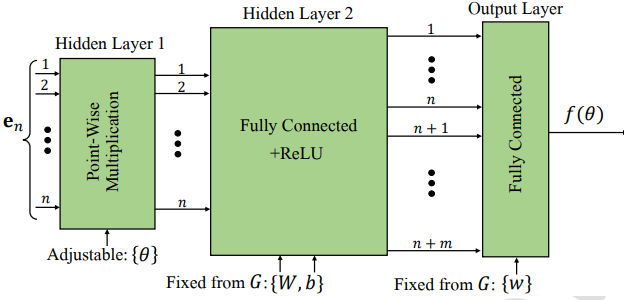
\includegraphics{figures/nn_block_structure.png}
    \caption{Scheme of proposed neural network $f(\theta)$}
    \label{fig:dnn_scheme}
\end{figure}

\begin{figure}[H]
    \centering
    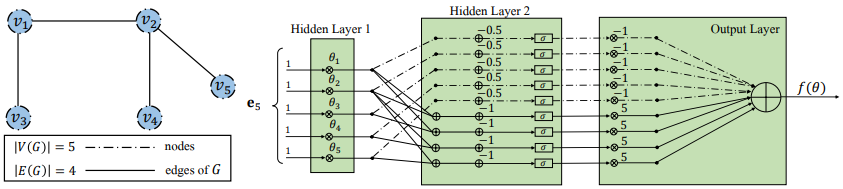
\includegraphics{figures/dnn_example.png}
    \caption{ An example of graph $G = (V = {v_1, v_2, v_3, v_4, v_5}, E =
{(v_1, v_2), (v_1, v_3), (v_2, v_4), (v_2, v_5)})$ and its dNN construction f for the MIS problem}
    \label{fig:dnn_example_1}
\end{figure}

\subsection{Loss function minimization techniques}
For minimization of the function and training the network we can use a few different approaches, like gradient descent, evolutionary minimization etc. 
 In our study we try to use both gradient descent approach and evolutionary minimization.
\subsubsection{Gradient descent}
 The main idea of gradient descent is to compute the gradient of the function and then apply a small step in the direction of the function minimization.
 For this it is relevant to imagine weights and biases stored as a 1-dimensional vector that we can call $\textbf{p} \in \mathbb{R}$.
Let the $\alpha (p):\mathbb{R}^s\ \longrightarrow \mathbb{R}$ be the loss function.
The process is iterative and involves computing a series of vectors in Rs with the goal of minimizing the loss function. Let us suppose that our current vector is \textbf{$p$}: how should we choose a perturbation,
$\delta p$, so that the next vector, $p+ \delta p$, represents an improvement? A Taylor series expansion
gives:
$$
\mathcal{L}(\mathbf{p}+\Delta \mathbf{p}) \approx \mathcal{L}(\mathbf{p})+\sum_{r=1}^s \frac{\partial \mathcal{L}(\mathbf{p})}{\partial p_r} \Delta p_r
$$
Here $ \frac{\partial \mathcal{L}(\mathbf{p})}{\partial p_r} $ stands for the partial derivative of the loss function with respect to $\textit{r}$-th parameter.  For convenience, we will let $\Delta \mathcal{L}(\mathbf{p}) \in \mathbb{R}^s$ denote the vector of partial derivatives,
known as the \textit{gradient}, so:
$$
\mathcal{L}(\mathbf{p}+\Delta \mathbf{p}) \approx \mathcal{L}(\mathbf{p})+\Delta \mathcal{L}(\mathbf{p})^T \Delta \mathbf{p}
$$
Our aim is to reduce the value of the loss function, so we should choose $\Delta \mathbf{p}$ to make $\Delta \mathcal{L}(\mathbf{p})^T \Delta \mathbf{p}$ as negative as possible. Hence, we should choose $\Delta \mathbf{p}$ to lie in the direction $-\Delta \mathcal{L}(\mathbf{p})$, limiting ourselves to a small step in that direction. This leads to the update:
$$
\mathbf{p} \longrightarrow \mathbf{p}-\eta \Delta \mathcal{L}(\mathbf{p})
$$
Here, $\eta$ is an optimization hyperparameter known as the learning rate, which controls the size of the step that the parameters take in the direction of the gradient.

However, when we have a large number of parameters and a large number of training points, computing the gradient vector at every iteration of the gradient descent method can be prohibitively expensive. A much cheaper alternative is to replace the mean of the individual gradients over all training points by the gradient at a single, randomly chosen, training point. This leads to the simplest form of what is called the stochastic gradient method (SGD) \ref{fig:gradient_descent}.

\begin{figure}[h]
    \centering
    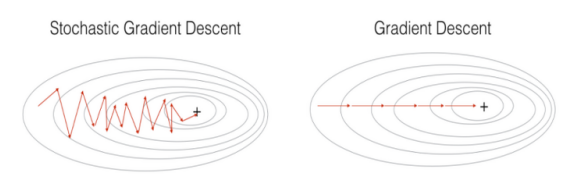
\includegraphics{figures/gradient_descent.png}
    \caption{Gradient descent}
    \label{fig:gradient_descent}
\end{figure}
 
 For gradient descent complexity of the algorithm depends on complexity of the gradient calculation. Noticing, that in network all parameters except $\theta$ are fixed, we can calculate only one gradient $\nabla |f(\theta) - f_d|^2$. Other parameters describe only the graph structure and are constant during the training procedure so they don't have to be updating by the gradient applying phase. 
 Thus, we iteratively minimize the loss function $\mathcal{L}(f(\theta),f_d)=|f(\theta)-f_d|^2$ by applying the gradient descent. 
 According to the Theorem \ref{minimum_f_value_theorem}, the minimum achievable value of $f(\theta)$ is a function of the cardinality of MIS. According to this, we set $f_d=n/2$ because we don't now what is the size of the MIS.

\subsubsection{Evolutionary minimization}

Because they ideally make no assumptions about the underlying fitness landscape, evolutionary algorithms frequently do well in approximating solutions to many kinds of problems. Planning models based on cellular processes and investigating microevolutionary processes are the main applications of evolutionary algorithms to the modeling of biological evolution. Computational complexity is a limiting issue in the majority of real-world implementations of EAs. Actually, the assessment of the fitness function is what causes this computational complexity. One method to get around this problem is to approximate fitness. There may not be a straight correlation between algorithm complexity and issue complexity, as seeming simplicity in EA can solve complicated problems frequently.

For our study we use a variant of \textbf{differential evolution}.

A basic variant of the DE algorithm works by having a population of candidate solutions (called agents). These agents are moved around in the search-space by using simple mathematical formulae to combine the positions of existing agents from the population. If the new position of an agent is an improvement then it is accepted and forms part of the population, otherwise the new position is simply discarded. The process is repeated and by doing so it is hoped, but not guaranteed, that a satisfactory solution will eventually be discovered.

Formally, let $f: \mathbb{R}^n \rightarrow \mathbb{R}$ be the fitness function which must be minimized (note that maximization can be performed by considering the function $h:=-f$ instead). The function takes a candidate solution as argument in the form of a vector of real numbers and produces a real number as output which indicates the fitness of the given candidate solution. The gradient of $f$ is not known. The goal is to find a solution $\mathbf{m}$ for which $f(\mathbf{m}) \leq f(\mathbf{p})$ for all $\mathbf{p}$ in the search-space, which means that $\mathbf{m}$ is the global minimum.

Let $\mathbf{x} \in \mathbb{R}^n$ designate a candidate solution (agent) in the population. The basic DE algorithm can then be described as follows:
\begin{enumerate}
\item Choose the parameters $\mathrm{NP} \geq 4, \mathrm{CR} \in[0,1]$, and $F \in[0,2]$
    \begin{enumerate}
        \item $\mathrm{NP}$ is the population size, i.e. the number of candidate agents or "parents"; a typical setting is $10 n$
        \item The parameter $\mathrm{CR} \in[0,1]$ is called the crossover probability and the parameter $F \in[0,2]$ is called the differential weight. Typical settings are $F=0.8$ and $C R=0.9$.
    \end{enumerate}
    \item Initialize all agents $\mathbf{x}$ with random positions in the search-space.
    \item Until a termination criterion is met (e.g. number of iterations performed, or adequate fitness reached), repeat the following:
    \begin{enumerate}
        \item Pick three agents $\mathbf{a}, \mathbf{b}$, and $\mathbf{c}$ from the population at random, they must be distinct from each other as well as from agent $\mathbf{x}$. (a is called the "base" vector.)
        \item Pick a random index $R \in\{1, \ldots, n\}$ where $n$ is the dimensionality of the problem being optimized.
        \item Compute the agent's potentially new position $\mathbf{y}=\left[y_1, \ldots, y_n\right]$ as follows:
        \begin{enumerate}
        \item For each $i \in\{1, \ldots, n\}$, pick a uniformly distributed random number $r_i \sim U(0,1)$
        \item If $r_i<C R$ or $i=R$ then set $y_i=a_i+F \times\left(b_i-c_i\right)$ otherwise set $y_i=x_i$. (Index position $R$ is replaced for certain.)
        \end{enumerate}
        \item If $f(\mathbf{y}) \leq f(\mathbf{x})$ then replace the agent $\mathbf{x}$ in the population with the improved or equal candidate solution $\mathbf{y}$
    \end{enumerate}
    \item Pick the agent from the population that has the best fitness and return it as the best found candidate solution.
\end{enumerate} 

 
\section{Exploiting the max clique problem in the neural network}
 
 We suggest including the edges of $G'$ since the graph generated by the MIS is a null graph on G and completely connected on its complement $G'$ to improve the tuning of the parameters during the construction of $f$. The resulting improved neural network is referred to as $h$ with output value $h(\theta)$. Given that we are changing the structure of the neural network, it is worth updating the variables responsible for the structure of the graph. Note: we do not change the overall structure of the layers or their quantity, we just update the sizes and value of the corresponding variables in the layers. In this case, sized of fixed parameters should be updated the next way: 
\begin{equation}
    W \in \{0,1\}^{n\cdot (n+m)} \longrightarrow W \in \{0,1\}^{n\cdot(n+m+m')}
\end{equation}
\begin{equation}
    b \in {-1,-1/2}^{n+m} \longrightarrow b \in \{-1,-1/2\}^{n+m+m'}
\end{equation}
\begin{equation}
    w \in \{-1,n\}^{n+m} \longrightarrow w \in \{-1,n\}^{n+m+m'}
\end{equation}
The values of the updated variables represent the structure of the complement graph $G'$ in such way:
\begin{equation}\label{W}
    W(i, n+m+l) = W(j,n+m+l)=1,\forall e_l=(v_i,v_j) \in E(G'),l\in[m']
\end{equation}
\begin{equation}\label{b}
    b(n+m+l)=-1,l\in [m']
\end{equation}
\begin{equation}\label{w}
    w(n+m+l)=-1,l\in[m']
\end{equation}
Taking into account the above changes, we obtain a new formula for the result of the neural network:
\begin{equation}
    h(\theta) = f(\theta) - \sum_{(u,v)\in E(G')} \sigma(\theta_u +\theta_v - 1)
\end{equation}

\begin{theorem}
\label{minimum_h_value_theorem}
Given a graph \graphG and it's adjusted neural network h, maximum independent set $I \subseteq V$ of $G$ has size $|I| = k \iff$ minimum value of $h$ is $-k^2/2$.
\end{theorem}
\begin{proof}
According to Theorem \ref{minimum_f_value_theorem} the minimum of $f$ is $-k/2$. So, we have to find the minimum value of the remaining term which belongs to $G'$. Let's assume that $\theta_v = 1 \forall v \in U$ and $\theta_v = 0$ in other cases. The induced by the MIS graph w.r.t $G'$ is fully connected graph, s.t. $|E(G'[U])|=k(k-1)/2$. If the bias is -1, the outputs corresponding $G'$ will be equal to 1. As the subgraph induced on $G'$ is complete, we obtain $-k(k-1)/2$ for the remaining term. Total result for $h$ is $-(k/2)-(k(k-1)/2)=-k^2/2$.
\end{proof}

Since the new minimum value for the network result $h$ is $-k^2/2$, we use $h_d=-n^2/2$ for minimization the network loss $\mathcal{L}(h(\theta),h_d)=|h(\theta)-h_d|^2$ because we do not know the size of the MIS.

Assuming that in graph \graphG vertices with high number of neighbours probably will not belong to MIS we can assign initial $\theta$ corresponding to the degree of vertices in order to increase the network convergence speed:
\begin{equation}
    \theta_v = 1 - \frac{d(v)}{\Delta(G)}
\end{equation}
Considering the fact that gradient descent applies the same gradient for all variables we add random small noise $s$ to each $\theta_i$ so training variables can by updated independently. Also, we have to notice that adding random positive noise to $\theta_v$ where corresponding vertex $v$ have no neighbors will make $\theta_v > 1$ that violates the constraint so initial weights should be clipped from 0 to 1.
\begin{equation} \label{theta}
    \hat{\theta}_v = 1 - \frac{d(v)}{\Delta(G)} + s, 
\end{equation}
\begin{equation*}
\theta_v = 
\begin{cases}
    1, \hat{\theta}_v > 1 \\
    \hat{\theta}_v, \hat{\theta}_v <=1
\end{cases}
\end{equation*}

For minimization of the function $h$ with box-constrained variables $\theta$ we use the ADAM stohastic gradient-based optimizer.
On each training iteration the obtained set $\mathcal{I}$ is checked whether it is maximal independent set by checking if a new node $v \in V, v \notin \mathcal{I}$ can be added to the set and there are no edges in the induced graph $E(G[\mathcal{I}]) = \varnothing$.

\begin{algorithm}[]
\caption{Neural network training}\label{alg:neural_network}
\begin{algorithmic}
\Function{$\mathcal{I}$}{$G,\alpha$}
    \State \textbf{construct} $h$ from $G$ using \ref{W}, \ref{b}, \ref{w}
    \State\textbf{initialize} $\theta$ using \ref{theta}, $\mathcal{I(\theta)=\varnothing}$
    \While {$\exists v \in V \textbackslash \mathcal{I}(\theta)$ s.t. $E[G(\mathcal{I}(\theta)\cup\{v\}) \neq \varnothing$ \textbf{OR} $E(G[\mathcal{I}]) \neq \varnothing$}
        \State \textbf{update} $\theta \leftarrow argmin_{\theta \in [0,1]^n}|h(\theta)-h_d|^2$
        \State \textbf{obtain} $\mathcal{I}(\theta)=\{v\in V | \theta_v \geq \alpha \}$
    \EndWhile
    \State \Return $\mathcal{I}$
\EndFunction
\end{algorithmic}
\end{algorithm}

The main problem of the presented neural network approach is it's RAM requirements for network construction. The largest part of the network is the matrix $W$ that has $n(n+m+m')$ elements. Thus, for dealing with large graphs (mainly MIS problem is hard to solve for large graphs, because for small ones the deterministic algorithms can be used) we propose graph reduction technique that split \graphG to subgraphs by communities and use dNN on graphs with reduced cardinality.
The scheme of the enhanced dataless neural network can be found on picture \ref{fig:dnn_clique_scheme}
\begin{figure}[h]
    \centering
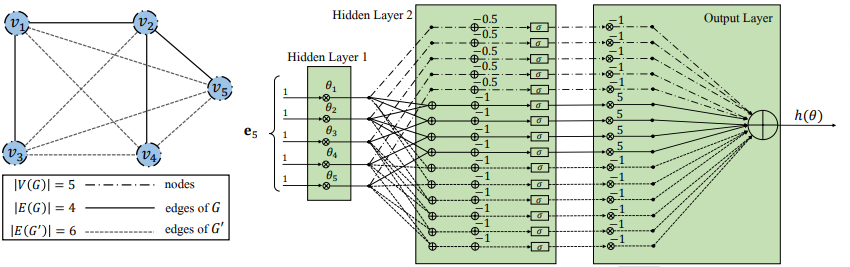
\includegraphics{figures/nn_clique_block_structure.png}
    \caption{An example of graph $G = (V = {v_1, v_2, v_3, v_4, v_5}, E =
{(v_1, v_2), (v_1, v_3), (v_2, v_4), (v_2, v_5)})$ and its dNN construction h for the MIS problem
by leveraging the duality between MIS and MC.
}
    \label{fig:dnn_clique_scheme}
\end{figure}

\section{Analysis of the large graphs}

Many techniques have been developed before to handle large-scale graphs for the MIS problem, such as the linear programming (LP) reduction, elimination of pendant vertices, and other heuristics as reported in \cite{butenko_applications} and used in some of the most recent state-of-the-art approaches. However, as mentioned in \cite{redumis}, these methods are only relevant to sparse graphs.

This inspires us to focus on creating a reduction method that is not dependent on the density or other properties of the graph. When handling big graphs, the suggested method detailed below makes use of dNNs, built on reduced subgraphs. This is especially helpful when optimizing the parameters of one dNN representing the complete graph necessitates a significant amount of storage and processing. 

To divide the graph into communities, which are made up of vertices with dense connections inside same community and sparser connections between communities, we perform Louvain community detection algorithm \cite{Yang2016}. 

The advancement of modularity in the algorithm serves as the model for this community discovery technique. The relative density of edges within communities compared to edges outside communities is measured using a scale called modularity, which ranges from 0.5 (non-modular clustering) to 1 (completely modular clustering). The best potential clustering of the nodes in a given network is achieved by optimizing this value, according to theory. Heuristic methods are utilized instead since it is difficult to iterate the nodes into groups across all potential configurations. In the Louvain Method of community discovery, each tiny community is initially grouped into one node and the first step is repeated until small communities are discovered by improving modularity locally on all nodes. The approach is comparable to an earlier approach developed by Clauset, Newman, and Moore that links communities whose merger results in the greatest gain in modularity.

Then, for the subgraph induced by each community separately, we generate a MIS using Algorithm \ref{alg:neural_network}. 

Let $C_i, i\in[r]$ be the set of nodes in community $i$, where $r$ - total quantity of communities in \graphG found by the community detection algorithm. For each $C_i$ we induce \graphG by $C_i$, $G_i=G[C_i]$. The union of these sets is the set $B = \bigcup_{i \in [r]} \mathcal{I_i}$
When all the communities are processed we obtain set of MIS $U = I$. Because there may be edges connecting nodes in the solution sets of two different communities, it should be noted that $B$ is typically not an independent set with respect to \graphG.

Thus, we call these edges forbidden and should replace or remove them from the solution.
Let's denote the inter-cluster edges:
\begin{equation}
    R = \{(u,v)\in E | u \in C_i, v \in C_j, i\neq j\}
\end{equation}

then, we can describe forbidden edges:
\begin{equation}
    F = \{(u,v) \in R | u \in \mathcal{I}_i, v \in \mathcal{I}_j, i \neq j\}
\end{equation}

We must handle every node having an edge in the set $F$ in order to get a MIS w.r.t. \graphG. In order to achieve this, we use the procedure below, which processes each pair in $F$ until an IS is obtained w.r.t. \graphG. Firstly, we choose a pair $(u, v) \in F$, and then determine if each node $q \in \{u, v\}$ may be substituted by a node in its neighborhood. A vertex $w \in N(q)$, is potential replacement if it is 1-tight, meaning that $|B\cap N(w)| = 1$. If neither $u$ nor $v$ can be replaced, the node in $F$ with the most repeats is eliminated. This procedure is continuing until the set $F$ is empty. Algorithm \ref{alg:forbiden_nodes_removal} provides the complete process. 

\begin{algorithm}
\caption{Forbidden nodes removal}\label{alg:forbiden_nodes_removal}
\begin{algorithmic}
\State \textbf{Input:}\graphG, $B$, $F$
\State \textbf{Output:} IS $\mathcal{I} on G$
\State \textbf{initialize} $\mathcal{I} = B$
\While{$F \neq \varnothing$}
    \State \textbf{select} a pair $(u,v) \in F,$ \textbf{initilize} ReplacementFlag = 0
    \State \textbf{for all} $q \in \{u,v\}$
    \If {$\exists w \in N(q)$ \textbf{s.t.} $|\mathcal{I}\cap N(w)| = 1$}
        \State \textbf{replace} $q$ by $w$, that is $\mathcal{I} \leftarrow \mathcal{I} \ \{q\}, \mathcal{I}\leftarrow \mathcal{I} \cup \{w\}$
        \State \textbf{update} $F$, ReplacementFlag = 1
        \State \textbf{break for}
    \EndIf
    \If {ReplacementFlag = 0 (no replacement is found)}
        \State \textbf{remove} either $u$ or $v$ depending on their repetitions in $F$
        \State \textbf{update} $\mathcal{I}$ and $F$
    \EndIf
\EndWhile
\end{algorithmic}
\end{algorithm}

Assuming that the resulting set $I$ is just an IS with respect to \graphG, we can create a MIS by applying Algorithm \ref{alg:neural_network} to the subgraph that is induced by nodes that are not part of the solution nor its neighborhood.
More strictly, result is updated as 
\begin{equation}
    \mathcal{I} \leftarrow \mathcal{I} \cup \text{dNN}(G[V\textbackslash(\mathcal{I} \cup N(\mathcal{I}))], \alpha)
\end{equation}

Example of the resulting independent sets for different small graphs can be found on figure \ref{figure:graphs_examples}
\begin{figure}
    \centering
  \begin{subfigure}{\linewidth}
  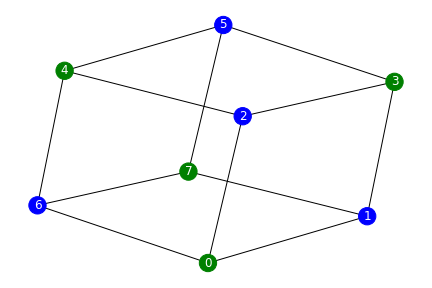
\includegraphics[width=.4\linewidth]{figures/small_graphs/1.png}
  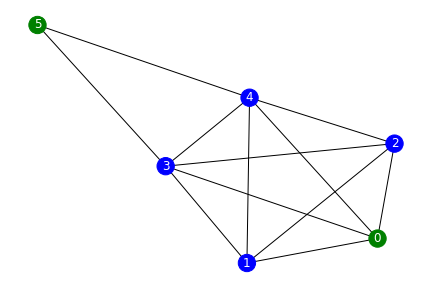
\includegraphics[width=.4\linewidth]{figures/small_graphs/2.png}
  \end{subfigure}\par\medskip
  \begin{subfigure}{\linewidth}
  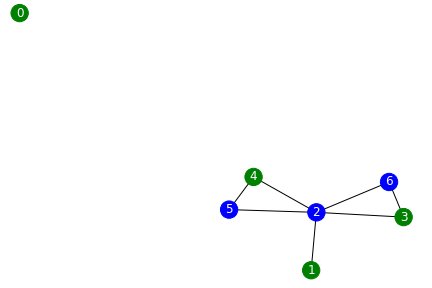
\includegraphics[width=.4\linewidth]{figures/small_graphs/3.png}
  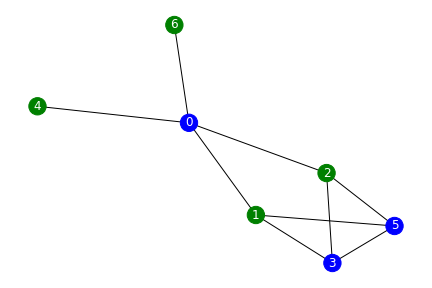
\includegraphics[width=.4\linewidth]{figures/small_graphs/4.png}
  \end{subfigure}\par\medskip
  \begin{subfigure}{\linewidth}
  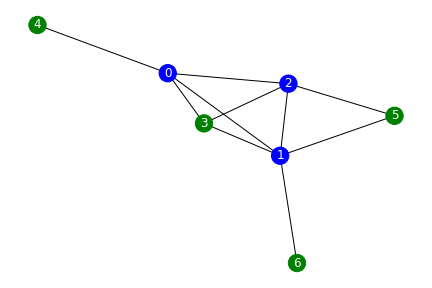
\includegraphics[width=.4\linewidth]{figures/small_graphs/5.png}
  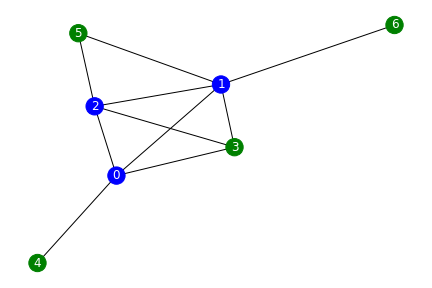
\includegraphics[width=.4\linewidth]{figures/small_graphs/6.png}
  \end{subfigure}\par\medskip
  \caption{Examples of MIS found for small graphs by the dNN algorithm. Vertices that are included to MIS are colored with green} \label{figure:graphs_examples}
\end{figure}


\chapter{Heuristical solution improvement}
\section{Preprocessing phase}
On preprocessing phase we can increase the quality of the dNN solution by applying a few simple technics exploiting the graph structure and relation between cliques and independent sets.
\subsection{Simplicial vertex reduction}
A \textbf{simplicial} vertex is one whose neighbors form a clique: every two neighbors are adjacent.  
In a graph $G$, a vertex $x$ is simplicial if its neighbourhood $N(x)$ induces a complete
subgraph of $G$. A graph is triangulated if it does not contain as an induced subgraph
a chordless cycle of length at least four (a \textit{hole}). A famous theorem of Dirac \cite{HOANG2004117} states
that every triangulated graph has a simplicial vertex. Let us also say that a vertex is
co-simplicial if its non-neighbours form an independent subset of vertices, and that a
graph is co-triangulated if it does not contain the complement of a chordless cycle on at least four vertices (an \textit{antihole}). Dirac’s theorem says equivalently that every
co-triangulated graph has a co-simplicial vertex. 
\begin{theorem}[Dirac]
Let $G$ be a triangulated graph. Then either $G$ is a clique or
$G$ contains two non-adjacent simplicial vertices.
\end{theorem}

Noticing that if a subgraph $S$ of \graphG forms a clique than there can only be one vertex in this subgraph that will be part of the MIS. By finding all the simplicial vertices in the $G$ we can add them to the $\mathcal{I}$ and remove them with their neighborhood from the initial graph. In such way we can use deterministic search and  reduce the cardinality of graph $G$ to be processed by the dNN and obtain part of the MIS. 
\begin{algorithm}[H]
\caption{Simplicial nodes search}\label{alg:simplicial-nodes-search}
\begin{algorithmic}
\Function{Simplicial nodes reduction}{$G$}
    \State $S = \varnothing$
    \State $NB = \varnothing$
    \For{$v \in V$}
        \If{$v \notin NB$}
            \State flag = 1
            \For{$q \in N(v)$}
                \For{$u \in N(v)$}
                    \If{$q \neq v$ and $\nexists e_{q,u}$}
                        \State flag = 0
                    \EndIf
                \EndFor
            \EndFor
            \If{flag = 1}
                \State $S \leftarrow S \cup v$
                \State $NB \leftarrow NB \cup N(v)$
            \EndIf
        \EndIf
    \EndFor
    \State $\hat{G} \leftarrow G[G\textbackslash (S \cup NB)]$
    \State \Return $S$, $\hat{G}$
\EndFunction
\end{algorithmic}
\end{algorithm}

\subsection{Linear programming reduction}

We exploit linear programming solution on graphs with low density (< 0.1) before community detection and applying dNN $h$. Minimization solution of 
\begin{equation}
    x^* = argmax \{\sum_{v\in V} x_v \text{ s.t. } x_v \geq 0, \forall v \in V, x_v + x_u \leq  1, \forall (u,v) \in E\}
\end{equation}

is obtained using linear programming solver built in $scipy$ python package. The vertices that belong to set $T = \{v \in V | {x^*}_v = 1\}$ must be in the MIS, so they can be removed from graph $G$ with their neighborhood $N(T)$. The solution $\mathcal{I}$ that is obtained after communities processing on $G[V\textbackslash(T\cup N(T))]$ and postprocessing phase can be joined with $T$ to obtain the MIS on $G$.

\section{Postprocessing phase}
To improve the solution of the dNN we utilize 2 simple technics on community and postprocessing phases - removing nodes with small degrees, and permutational maximization with local search.

\subsection{Small degrees vertices reduction}
Given graph G and solution I, we present a solution improvement technique that eliminates a group of low-degree nodes $U \in \mathcal{I}$, such that $|U| =,\lambda$ together with their neighbors $N(U)$ from the graph since high-degree nodes are less likely to be in a big IS. After that we apply our dNN to the smaller graph $G[V\textbackslash (U \cap N(U))$. This process is applied iteratively, increasing $\lambda$ with each iteration. Up until a certain stopping criterion is met, the best solution is retained. 

\begin{algorithm}
\caption{Low-degree vertices excluding}\label{alg:log-degree-vertices-excluding}
\begin{algorithmic}
\State \textbf{Input:} \graphG, Solution $\mathcal{I},\lambda, IncreaseStep$
\State \textbf{Output:} $\mathcal{I}^*$
\State \textbf{initialize:} $\mathcal{I}^* = \mathcal{I}$
\While{stopping criteria is not satisfied}
    \State \textbf{obtain} $U \subset \mathcal{I}:|U|=\lambda,\forall u \in U, v \in \mathcal{I}  U,d(u) \leq d(v)$
    \State \textbf{obtain} $\mathcal{I}\leftarrow \mathcal{I}\cup \text{dNN}(G[V\textbackslash(U\cup N(U))],\alpha)$
    \If{$|\mathcal{I}| > |\mathcal{I^*}|$ (update the optimum if $\mathcal{I}$ has higher cardinality) }
        \State \textbf{update} $\mathcal{I}^* = \mathcal{I}$ 
    \EndIf
    \If{$|\mathcal{I}| \leq |\mathcal{I^*}|$ (restart from the current optimum) }
        \State \textbf{update} $\mathcal{I} = \mathcal{I}^*$ 
    \EndIf
    \State \textbf{update} $\lambda \leftarrow \lambda + IncreaseStep$
\EndWhile
\end{algorithmic}
\end{algorithm}

After the tests, we decided that it is reasonable to set initial $\lambda$ to 5 and finish iterations when the cardinality of the new-obtained graph $G[V\textbackslash(U\cup N(U))]$ is less then 20. 

The number of computations required for Algorithm \ref{alg:log-degree-vertices-excluding} depends on $\lambda$ and the
rate by which it increases as this determines the size of the subgraph on which the $dNN$ procedure is applied on each iteration.

\subsection{Local search improvement}
The most effective methodology for designing MIS heuristics is local search. In our case we use the next 2-improvement algorithm \cite{local-search} to increase the size of the MIS during the postprocessing phase when all the communities are processed.

For a vertex$v, v\notin \mathcal{I}$ let's call \textbf{tightness} ($\tau(v)$) of $v$ w.r.t $\mathcal{I}$ the quantity of neighbors of $v$ that belong to $\mathcal{I}$. If the vertex $v$ has tightness of 0, we call it a \textbf{free} vertex.
It is obvious that if node $v$ belongs to $\mathcal{I}$ and $\exists q, q \in N(v), \tau(q) = 1$ than the only neighbour of $q$ that belongs to $\mathcal{I}$ is $v$.

We construct a data structure $X$ that consists of 3 groups of vertices in $V$ w.r.t $\mathcal{I}$:
\begin{itemize}
    \item free nodes in $V$
    \item non-free nodes in $V$
    \item nodes that belong to $\mathcal{I}$
\end{itemize}

During the iteration of the algorithm if there are any free nodes we add 1 node of them to $\mathcal{I}$ and recompute $X$. If there are no free nodes in $X$ we try to find a node $v \in \mathcal{I}$, s.t. there are at least to nodes in it's neighbors s.t. their tightness is equal to exactly 1 and they don't have edge between them: $q,u \in N(v), \tau(q) = \tau(v) = 1, E[(q,u)] = \varnothing$. For this we calculate the tightness of the all non-free nodes and if their tightness is equal to 1 we add them to a map, grouped by vertex$v \in \mathcal{I}$. If such 2 neighbors $q,u$ of node $v$ are found and there is no edges between them we can remove node $v$ from $\mathcal{I}$ and add $q,v$ to $\mathcal{I}$ increasing the size of $\mathcal{I}$ by 1. After this we recompute $X$.
We repeat this algorithm until there are no free nodes no pair of 1-tightness neighbors left in $X$. 


\chapter{Computational results}
The algorithm was implemented using Python 3, tensorflow 2.9.1 and scipy 1.9.3. In this part we compare our proposed solver to the state-of-art ReduMIS solver.
Tests include search of the MIS on generated graphs and on DIMACS graphs. All results are compared to the state-of-art ReduMIS algorithm built with GNU C++ in terms of accuracy and execution time. Tests are executed on Intel(R) Core(TM) i7-6700HQ CPU @ 2.60GHz in single thread.

\subsection{Generated graphs results}
We test network on randomly generated higher-density graphs using from the Erdos-Renyi (ER) \cite{er60}, Barbosi-Albert (BA) \cite{ab02}, Holme and Kim (HK) \cite{hk02}, and the Stochastic Block (SBM) \cite{hll83} models.

\begin{table}[!ht]
    \centering
    \begin{tabular}{|l|l|l|l|l|l|}
    \hline
        \textbf{Graph} & \textbf{V} & \textbf{E} & \textbf{dNN result} & \textbf{ReduMIS result} & \textbf{Accuracy} \\ \hline
        \textbf{ER} & 100 (p = 0.1) & 500,00 & 28,15 & 30,50 & 0,92295082 \\ \hline
        \textbf{ER} & 100  (p = 0.2) & 983,00 & 18,00 & 20,00 & 0,9 \\ \hline
        \textbf{ER} & 200  (p = 0.1) & 2004,00 & 35,90 & 41,00 & 0,875609756 \\ \hline
        \textbf{ER} & 200  (p = 0.2) & 4000,00 & 20,00 & 25,50 & 0,784313725 \\ \hline
        \textbf{SBM} & 250  (p = 0.1) & 1874,00 & 55,50 & 61,00 & 0,909836066 \\ \hline
        \textbf{SBM} & 250  (p = 0.2) & 2481,00 & 45,90 & 51,00 & 0,9 \\ \hline
        \textbf{SBM} & 350  (p = 0.1) & 3666,00 & 63,10 & 68,00 & 0,927941176 \\ \hline
        \textbf{SBM} & 350  (p = 0.2) & 4883,00 & 51,60 & 55,50 & 0,92972973 \\ \hline
        \textbf{BA} & 100 & 2475,00 & 45,00 & 45,00 & 1 \\ \hline
        \textbf{BA} & 200 & 9950,00 & 95,00 & 95,00 & 1 \\ \hline
        \textbf{HK} & 100 & 2017,00 & 30,00 & 30,00 & 1 \\ \hline
        \textbf{HK} & 200 & 8092,00 & 60,00 & 60,00 & 1 \\ \hline
    \end{tabular}
    \caption{Dataless neural network result comparison with state-of-art ReduMIS solver}
    \label{table:generated_graphs_result}
\end{table}

For testing we also use DIMACS benchmark. The 1990s saw the creation of the DIMACS benchmark set for the second DIMACS challenge on Clique, Satisfiability, and Graph Coloring (Johnson \& Trick, 1996). It consists of 80 graphs and is the benchmark set for assessing MCP algorithms. The benchmark includes several real-world issues, including coding theory, fault diagnosis issues, Keller's hypothesis, and others, in addition to randomly generated networks and graphs in which the largest clique is concealed by using low-degree vertices.

On the figure \ref{fig:heuristic_algorithms_description} we can see description of the some most efficient heurstic algorithms for the MIS problem. On the table \ref{table:heuristic_algorithms_results} and \ref{table:heuristic_algorithms_performance} the average accuracy and performance of these algorithms is presented for the MIS problem on DIMACS graphs.
\begin{figure}[h]
    \centering
    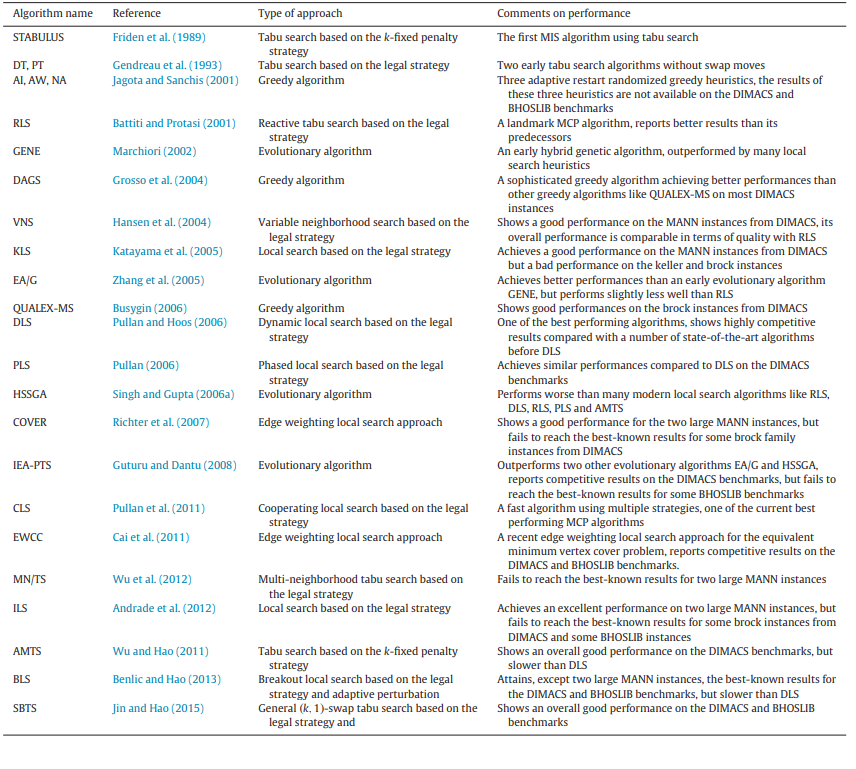
\includegraphics{figures/heuristic_algorithms_description.png}
    \caption{Best existing heuristic algorithms for MIS problem with description}
    \label{fig:heuristic_algorithms_description}
\end{figure}

\begin{table}[!ht]
    \centering
    \begin{tabular}{|l|l|l|l|l|l|l|}
    \hline
        \textbf{Instance} & \textbf{brock400\_2} & \textbf{brock800\_2} & \textbf{C2000.9} & \textbf{C4000.5} & \textbf{keller6} & \textbf{MANN\_a81} \\ \hline
        \textbf{RLS} & 29(26.06) & 21 & 78(77.58) & 18 & 59 & 1098 \\ \hline
        \textbf{GENE} & 24(22.5) & 20(19.3) & 72(68.2) & 16(15.4) & 55(51.8) & 1097(1096.3) \\ \hline
        \textbf{DAGS} & 29(28.10) & 24(20.82) & 76(75.40) & 18(17.50) & 57(56.40) & ~ \\ \hline
        \textbf{VNS} & 29(27.4) & 21 & 78(77.2) & 18 & 59(58.2) & 1100(1099.3) \\ \hline
        \textbf{KLS} & 25(24.84) & 21(20.86) & 77(74.90) & 18(17.02) & 57(55.59) & 1100(1098.07) \\ \hline
        \textbf{EA/G} & 25(24.7) & 21(20.1) & 72(70.9) & 17(16.1) & 56(53.4) & 1098(1097.2) \\ \hline
        \textbf{QUALEX-MS} & 29 & 24 & 72 & 17 & 53 & 1096 \\ \hline
        \textbf{DLS} & 29 & 24 & 78(77.93) & 18 & 59 & 1098(1097.96) \\ \hline
        \textbf{PLS} & 29 & 24 & 78 & 18 & 59(57.75) & 1098 \\ \hline
        \textbf{HSSGA} & 29(25.1) & 21(20.7) & 74(71.0) & 17(16.8) & 57(54.2) & 1095(1094.2) \\ \hline
        \textbf{COVER} & 28(-) & - & 78(77.84) & 18 & 59 & 1100(-) \\ \hline
        \textbf{IEA-PTS} & 29(27.52) & 24(21.06) & 79(76.4) & 18(17.66) & 59(57.06) & 1099(1097.01) \\ \hline
        \textbf{CLS} & 29 & 24 & 78 & 18 & 59 & 1098 \\ \hline
        \textbf{EWCC} & 29(25.48) & 21 & 79(78.56) & 18 & 59 & 1100(1098.11) \\ \hline
        \textbf{MN/TS} & 29 & 24(23.88) & 80(78.37) & 18 & 59 & 1090 \\ \hline
        \textbf{ILS} & 25 & 21 & 77(76.9) & 18(17.1) & 59 & 1100 \\ \hline
        \textbf{AMTS} & 29 & 24 & 80(78.95) & 18 & 59 & 1098 \\ \hline
        \textbf{BLS} & 29 & 24(23.04) & 80(78.6) & 18 & 59 & 1094(1092.17) \\ \hline
        \textbf{SBTS} & 29 & 24(22.29) & 80(77.29) & 18 & 59 & 1100 \\ \hline
    \end{tabular}
    \caption{Best and average results on the heuristic algorithms for MIS problem on DIMACS graphs}
    \label{table:heuristic_algorithms_results}
\end{table}

\begin{table}[!ht]
    \centering
    \begin{tabular}{|l|l|l|l|l|l|l|}
    \hline
        \textbf{Instance} & \textbf{brock400\_2} & \textbf{brock800\_2} & \textbf{C2000.9} & \textbf{C4000.5} & \textbf{MANN\_a81} & \textbf{keller6} \\ \hline
        \textbf{RLS} & 3.06 & 0.34 & 59.83 & 158.65 & 205.72 & 13.7 \\ \hline
        \textbf{GENE} & 0.27 & 0.75 & 4.89 & 1.95 & 401.41 & 8.7 \\ \hline
        \textbf{DAGS} & 0.62 & 3.73 & 405.33 & 717.55 & - & 2739.1 \\ \hline
        \textbf{VNS} & 4.17 & 0.85 & 22.74 & 310.71 & 65.47 & 17.9 \\ \hline
        \textbf{KLS} & 0.04 & 0.16 & 4.80 & 7.76 & 12.88 & 17,0 \\ \hline
        \textbf{EA/G} & 1.42 & 3.42 & 17.38 & 23.46 & 319.04 & 24.2 \\ \hline
        \textbf{QUALEX-MS} & 0.67 & 4.00 & 47.78 & 521.11 & 106.00 & 286.8 \\ \hline
        \textbf{DLS} & 0.12 & 3.97 & 48.79 & 45.76 & 66.66 & 43.0 \\ \hline
        \textbf{PLS} & 0.12 & 4.08 & 50.11 & 47.01 & 172.17 & 172.1 \\ \hline
        \textbf{HSSGA} & 0.14 & 1.35 & 14.83 & 19.97 & 503.99 & 39.6 \\ \hline
        \textbf{COVER} & - & ~ & 139.36 & 260.27 & - & 5.8 \\ \hline
        \textbf{IEA-PTS} & 1.08 & 1.03 & 19.71 & 104.21 & 237.55 & 45.4 \\ \hline
        \textbf{CLS} & 0.08 & 1.73 & 7.28 & 13.63 & 20.80 & 0.9 \\ \hline
        \textbf{EWCC} & 374.52 & 0.49 & 858.73 & 738.91 & 634.46 & 3.7 \\ \hline
        \textbf{MN/TS} & 0.81 & 94.25 & 339.57 & 86.96 & 380.87 & 58.9 \\ \hline
        \textbf{ILS} & 11.57 & 63.15 & 108.42 & 1996.84 & 10.52 & 546.3 \\ \hline
        \textbf{AMTS} & 0.69 & 19.61 & 266.33 & 74.93 & 16.30 & 6.3 \\ \hline
        \textbf{BLS} & 10.29 & 637.94 & 2846.84 & 387.33 & - & 14.6 \\ \hline
        \textbf{SBTS} & 11.97 & 464.12 & 896.78 & 919.07 & 13.43 & 446.6 \\ \hline
    \end{tabular}
    \caption{Heuristic algorithms time performance (in seconds) on DIMACS graphs}
    \label{table:heuristic_algorithms_performance}
\end{table}

TODO: Add evolutionary minimization/gradient comparison.

%   BACK MATTER
%   BIBLIOGRAPHY
\cleardoublepage
\addcontentsline{toc}{chapter}{bibliography}
\bibliography{include/3-back/bibliography}

%   APPENDIX
\cleardoublepage
\appendix % to tell LaTeX that the following chapters are appendices
\renewcommand\chaptername{Appendix}
\chapter{Dataless network implementation}
\begin{lstlisting}
import gc
import logging
import os
import matplotlib.pyplot as plt
import networkx as nx
import networkx.algorithms.community as nx_comm
import numpy as np
import random
import scipy
from scipy.optimize import differential_evolution, linprog
import tensorflow as tf
import time
import warnings

class DnnResult():
    def __init__(self, theta, stuck):
        self.theta = theta
        self.stuck = stuck

class ValidationResult():
    def __init__(self, valid, can_add_nodes, contains_extra_nodes):
        self.valid = valid
        self.can_add_nodes = can_add_nodes
        self.contains_extra_nodes = contains_extra_nodes 

def clip(l,r,x):
    return max(l,min(r,x))

def calc_W(G, C):
    n = len(G.nodes())
    m = len(G.edges())
    m_c = len(C.edges())
    W = np.zeros((n,n+m+m_c),dtype= 'float32')
    for i in range(n):
        W[i][i] = 1
    j = n
    for edge in G.edges():
        x = int(edge[0])
        y = int(edge[1])
        W[x][j] = 1
        W[y][j] = 1
        j+=1
    for edge in C.edges():
        x = int(edge[0])
        y = int(edge[1])
        W[x][j] = 1
        W[y][j] = 1
        j+=1
    return W

def calc_b(G, C):
    n = len(G.nodes())
    m = len(G.edges())
    m_c = len(C.edges())
    b = np.array([-1/2 for i in range(n)])
    b_m = np.array([-1 for i in range(m+m_c)])
    return np.concatenate((b,b_m))

def calc_w(G, C):
    n = len(G.nodes())
    m = len(G.edges())
    m_c = len(C.edges())
    w = np.array([-1 for i in range(n)])
    w_n = np.array([n for i in range(m)])
    w_c = np.array([-1 for i in range(m_c)])
    return np.concatenate((w,w_n,w_c))

def build_theta(G):
    n = len(G.nodes())
    max_degree = max([G.degree(i) for i in range(n)])
    if max_degree == 0:
        return np.array([1 for i in range(n)])
    return np.array([clip(0,1,1 - G.degree(i)/max_degree + random.random()/10000) for i in range(n)])

def build_network(G):
    logging.debug("Build network on graph G:{}.".format(str(G)))
    C = nx.complement(G)
    W = calc_W(G, C)
    b = calc_b(G, C)
    w = calc_w(G, C)
    theta = build_theta(G)
    return (W,b,w, theta, C)

def get_result_nodes(theta, alpha = 0.5):
    return set(np.argwhere(theta > alpha).reshape(-1))

def not_connected_nodes_exist_in_G(G, result_nodes):
    for v in G.nodes():
        if v not in result_nodes:
            node_not_connected_to_G = True
            for edge in G.neighbors(v):
                if edge in result_nodes:
                    node_not_connected_to_G = False
                    break
            if node_not_connected_to_G:
                return True
    return False
            
def graph_has_no_edges(G, result_nodes):
    for v in result_nodes:
        for edge in G.neighbors(v):
            if edge in result_nodes:
                return False
    return True

def mis_is_valid(G, mis):
    has_extra_nodes = not graph_has_no_edges(G, mis)
    not_connected_nodes_exist = not_connected_nodes_exist_in_G(G, mis)
    return ValidationResult(not has_extra_nodes and not not_connected_nodes_exist,
                            not_connected_nodes_exist, has_extra_nodes)
               
def result_is_valid(G, theta):
    result_nodes = get_result_nodes(theta)
    return mis_is_valid(G, result_nodes).valid

def network(theta,e_n,W_t,b,w_t):
    h = tf.math.multiply(e_n,theta)
    h = tf.linalg.matvec(W_t,h)
    h = tf.add(h,b)
    h = tf.nn.relu(h)
    h = tf.tensordot(w_t,h, 1)
    return h
    
def network_evol(theta,e_n,W_t,b,w_t):
    return network(theta,e_n,W_t,b,w_t).numpy()

def loss(theta,e_n,W_t,b,w_t,h_d):
    h = network(theta,e_n,W_t,b,w_t)
    diff = (h-h_d)**2   
    return diff

def loss_evol(theta,e_n,W_t,b,w_t,h_d):
    h = network_evol(theta,e_n,W_t,b,w_t)
    return (h-h_d)**2  

def evolutionary_train(n,theta,e_n,W_t,b,w_t,h_d):
    bounds = [(0,1) for i in range(n)]
    theta = differential_evolution(loss_evol, bounds, x0 = theta, args = (e_n,W_t,b,w_t,h_d))
    theta = theta.x
    return DnnResult(theta, False)

def vectors_are_close(a,b):
    norm_diff = np.linalg.norm(a-b)
    return norm_diff < 1e-6 

def gradient_train(G, max_epochs, theta,e_n,W_t,b,w_t,h_d):
    epoch = 0
    def local_loss():
        return loss(theta,e_n,W_t,b,w_t,h_d)
    optimizer=tf.optimizers.Adam(learning_rate=0.1,)
    var_list = theta
    solver_stuck = False
    previous_theta = np.copy(theta.numpy())
    while not result_is_valid(G, theta) and epoch < max_epochs and not solver_stuck:
        optimizer.minimize(local_loss, var_list=var_list)
        epoch+=1
        if np.allclose(previous_theta, theta.numpy()):
            solver_stuck = True
        previous_theta = np.copy(theta.numpy())
    return DnnResult(theta.numpy(),solver_stuck or epoch == max_epochs)

def train_network(G, max_epochs, method="gradient"):
    (W,b,w, theta, C) = build_network(G)
    n = len(G.nodes())
    W_t = tf.constant(W.T, dtype = 'float32')
    b = tf.constant(b, dtype = 'float32')
    w_t = tf.constant(w.T, dtype = 'float32')
    theta = tf.Variable(theta,
                        trainable=True,
                        constraint = lambda x: tf.clip_by_value(theta,0,1),
                        dtype = 'float32')
    e_n = tf.constant(np.ones((n)),dtype = 'float32')
    h_d = tf.constant(-n*n/2,dtype = 'float32') 

    if method == "evolutionary":
        result = evolutionary_train(n,theta, e_n,W_t,b,w_t,h_d)
    elif method == "gradient":
        result = gradient_train(G, max_epochs,theta, e_n,W_t,b,w_t,h_d)
    return result

def find_inter_cluster_edges(G, communities):
    edges = dict()
    for com in communities:
        for node_i in communities[com]:
            for neighbour_i in G.neighbors(node_i):
                if neighbour_i not in communities[com]:
                    if edges.get(node_i) is not None:
                        edges[node_i].add(neighbour_i)
                    else:
                        edges[node_i] = {neighbour_i}
                    if edges.get(neighbour_i) is not None:
                        edges[neighbour_i].add(node_i)
                    else:
                        edges[neighbour_i] = {node_i}
    return edges

def find_forbidden_edges(G, R, independent_sets):
    forbidden = []
    for u, edges in R.items():
        if u in independent_sets:
            for v in edges:
                if v in independent_sets:
                    forbidden.append((u, v))
    return forbidden
    
def collect_list_by_dicts_key(partitions):
    communities = {}
    for key, val in partitions.items():
        if communities.get(val) == None:
            communities[val] = [key]
        else:
            communities[val].append(key)
    return communities

def collect_communities_to_map(communities):
    new_com = {}
    index = 0
    for com in communities:
        new_com[index] = com
        index+=1
    return new_com

def build_G_from_nodes(G, nodes):
    communities = {}
    N = len(nodes)
    new_G = nx.Graph()
    index_map = dict()
    node_map = dict()
    index = 0
    for node in nodes:
        index_map[index] = node
        node_map[node] = index
        new_G.add_node(index)
        index+=1
    for i in nodes:
        for j in nodes:
            if G.has_edge(i,j):
                new_G.add_edge(node_map[i], node_map[j])
                new_G.add_edge(node_map[j], node_map[i])
    return (new_G, index_map, node_map)

def node_is_new_candidate(G, node, mis):
    for w in G.neighbors(node):
        neighbors_in_mis_count = 0
        if w not in mis:
            for n_w in G.neighbors(w):
                if n_w in mis:
                    neighbors_in_mis_count += 1
                    if neighbors_in_mis_count == 2:
                        break
            if neighbors_in_mis_count == 1:
                return (True, w)
    return (False, -1) 

def get_node_with_most_occurences(F):
    count_dict = dict()
    for edge in F:
        for node in edge:
            if node in count_dict:
                count_dict[node]+=1
            else:
                count_dict[node]=0
    maximum = 0
    max_node = None
    for node in count_dict:
        if count_dict[node] > maximum:
            max_node = node
    return node

def replace_node_if_possible(G,F,mis,node):
    (can_be_replaced, new_node) = node_is_new_candidate(G,node,mis)
    if can_be_replaced:
        mis.remove(node)
        mis.add(new_node)
        return True
    return False 

def replace_forbiden_nodes(G,R,F,mis):
    while len(F) > 0:
        replaced = False
        for edge in F:
            for node in edge:
                replaced = replace_node_if_possible(G,F,mis,node)
                if replaced:
                    break
            if replaced:
                break
        if not replaced:
            node_to_be_removed = get_node_with_most_occurences(F)
            mis.remove(node_to_be_removed)
        F = find_forbidden_edges(G, R, mis)
    return mis

def build_G_from_left_nodes(G, nodes):
    mis_with_neighbours = set()
    for node in nodes:
        mis_with_neighbours.add(node)
        for neighbour in G.neighbors(node):
            mis_with_neighbours.add(neighbour)
    nodes_left_to_process = set(G.nodes()).difference(mis_with_neighbours)
    return build_G_from_nodes(G,nodes_left_to_process)

def calculate_mis_with_left_nodes(G, mis_list, max_epochs,method):
    (left_G, left_index_map, left_node_map)  = build_G_from_left_nodes(G, mis_list)
    if len(left_G.nodes()) > 100:
        mis = calculate_large_G(left_G, max_epochs)
    elif len(left_G.nodes()) > 0:
        mis = validate_dnn_result(train_network(left_G, max_epochs,method),left_G)
    else:
        mis = {}
    mis_correct = [left_index_map[node] for node in mis]
    mis_final = mis_list.union(mis_correct)
    return mis_final

def build_U_from_IS(_lambda, IS,G,):
    if len(IS) == 0:
        return []
    degree_list_ascending = [(G.degree(node),node) for node in IS]
    degree_list_ascending.sort(key=lambda pair: pair[0])
    return [pair[1] for pair in degree_list_ascending[:min(_lambda, len(IS))]]

def validate_dnn_result(dnn_result, G):
    if dnn_result.stuck:
       if len(G.edges()) < 50:
            mis = local_improvement(G,[0])
        else:
            communities = collect_communities_to_map(nx_comm.louvain_communities(G, resolution = 1.3, seed=seed))
            if len(communities) > 1:
                mis = calculate_large_G(G, resolution = 1.3)
            else:
                mis = nx.maximal_independent_set(G)
        dnn_result_nodes = get_result_nodes(dnn_result.theta)
        if len(dnn_result_nodes) > len(mis) and result_is_valid(G, dnn_result.theta):
            return dnn_result_nodes
        else:
            return mis
    else:
        theta_for_small_G = dnn_result.theta
        mis = get_result_nodes(theta_for_small_G)
        return mis

def try_remove_nodes_with_small_degree(I, G, max_epochs, method):
    _lambda = 5
    I_star = I
    index = 0
    while True:
        U = build_U_from_IS(_lambda, I_star,G)
        (reduced_G,index_map, node_map) = build_G_from_left_nodes(G, U)
        if len(reduced_G.nodes()) < 20:
            break
        index+=1
        dnn_result = train_network(reduced_G, max_epochs,method)
        mis_correct = {index_map[node] for node in validate_dnn_result(dnn_result, reduced_G)}
        I = set(I).union(U)
        if(len(I)>len(I_star)):
            I_star = I
        else:
            I = I_star
        _lambda+=1
    return I_star

def nodes_must_be_in_mis(G):
    n = len(G.nodes())
    m = len(G.edges())
    v_0 = [0 for i in range(n)]
    v_1_2 = [0.5 for i in range(n)]
    v_1 = [1 for i in range(n)]
    x_bound = [(0, 1) for i in range(n)]
    c = [-1 for i in range(n)]
    A = []
    b=[]
    for (u,v) in G.edges():
        u = int(u)
        v = int(v)
        if u < v:
            con = [0 for i in range(n)]
            con[u] = 1
            con[v] = 1
            A.append(con)
            b.append(1)
    res = linprog(c, A_ub=A, b_ub=b, bounds=x_bound,method='highs',)
    nodes_that_must_be_in_mis = set()
    for i in range(n):
        if abs(res.x[i]-1)<0.001:
            nodes_that_must_be_in_mis.add(i)
    return nodes_that_must_be_in_mis

def nodes_that_are_clique(G):
    cliques = set()
    clique_neighbors = set()
    for node in G.nodes():
        if node not in clique_neighbors:
            is_clique = True
            neighbors = set(G.neighbors(node))
            for n1 in neighbors:
                for n2 in neighbors:
                    if n1!=n2 and not G.has_edge(n1,n2):
                        is_clique = False
            if is_clique:
                clique_neighbors.update(neighbors)
                cliques.add(node)
    return cliques

def process_community(G, max_epochs, method, resolution, file_suffix):
    dnn_result = train_network(G, max_epochs,method)
    mis = validate_dnn_result(dnn_result, G)
    log_error_if_mis_is_wrong(G, mis)
    mis = try_remove_nodes_with_small_degree(mis, G, max_epochs, method)
    log_error_if_mis_is_wrong(G, mis)
    return mis

def process_main_algo(G, max_epochs, method, resolution, file_suffix):
    communities = collect_communities_to_map(nx_comm.louvain_communities(G, resolution, seed=seed))
    
    mis_list = set()
    community_index = 1
    write_G_to_file_in_metis_format(G,  "KaMIS/deploy/"+file_suffix)
    
    for com in communities:
        (G_com,index_map, node_map) = build_G_from_nodes(G, communities[com])
        
        write_G_to_file_in_metis_format(G_com,  "KaMIS/deploy/"+file_suffix+"community_" + str(com) )
        mis_com = process_community(G_com, max_epochs, method, resolution, file_suffix)
        mis_correct = {index_map[node] for node in mis_com}
        
        mis_list = mis_list.union(mis_correct)        
        community_index += 1
        
    R = find_inter_cluster_edges(G, communities)
    F = find_forbidden_edges(G, R, mis_list)
    replace_forbiden_nodes(G,R,F,mis_list)
    mis_list = calculate_mis_with_left_nodes(G, mis_list, max_epochs,method)
    log_error_if_mis_is_wrong(G, mis_list)
    return mis_list

def process_lp(G, max_epochs, method, resolution, file_suffix):
    density = nx.density(G)
    should_use_lp = density < 0.1
    G_before_LP = G
    if should_use_lp:
        nodes_from_lp_solver = nodes_must_be_in_mis(G)
        (G, index_map,_) = build_G_from_left_nodes(G, nodes_from_lp_solver)
        if len(G.nodes()) == 0:
            log_error_if_mis_is_wrong(G_before_LP, nodes_from_lp_solver)
            return nodes_from_lp_solver
    mis_list = process_main_algo(G, max_epochs, method, resolution, file_suffix)
    if should_use_lp:
        mis_list = {index_map[node] for node in mis_list}
        mis_list = mis_list.union(nodes_from_lp_solver)
    log_error_if_mis_is_wrong(G_before_LP, mis_list)
    return mis_list
def process_cliques(G, max_epochs, method, resolution, file_suffix):
    G_before_cliques = G
    cliques = nodes_that_are_clique(G)
    (G, cliques_index_map,_) = build_G_from_left_nodes(G, cliques)
    if len(G.nodes()) == 0:
        log_error_if_mis_is_wrong(initial_G, cliques)
        return cliques
    mis_list=process_lp(G, max_epochs, method, resolution, file_suffix)
    mis_list = {cliques_index_map[node] for node in mis_list}
    mis_list = mis_list.union(cliques)
    log_error_if_mis_is_wrong(G_before_cliques, mis_list)
    return mis_list

def local_improvement(G, mis):
    should_recalculate = True
    mis_flags = [0 for node in G.nodes()]
    for node in G.nodes():
        if node in mis:
            mis_flags[node] = 1
    while should_recalculate:
        L = [[] for i in range(len(mis_flags))]
        for node in G.nodes():
            if mis_flags[node] == 1:
                for n in G.neighbors(node):
                    tight = 0
                    for k in G.neighbors(n):
                        if mis_flags[k] == 1:
                            tight+=1
                    if tight == 1:
                        L[node].append(n)
                L[node].sort()
        
        for x in range(len(mis_flags)):
            if mis_flags[x] == 1:
                replaced = False
                if len(L[x]) > 1:
                    for v in L[x]:
                        for w in L[x]:
                            if v < w and not G.has_edge(v,w):
                                mis_flags[x] = 0
                                mis_flags[v] = 1
                                mis_flags[w] = 1
                                replaced = True
                                break
                        if replaced:
                            break
                    if replaced:
                            break
        if not replaced:
            for node in G.nodes():
                if mis_flags[node] == 0:
                    node_is_free = True
                    for neigh in G.neighbors(node):
                        if mis_flags[neigh] == 1:
                            node_is_free = False
                    if node_is_free:
                        replaced = True
                        mis_flags[node] = 1
                        break
        should_recalculate = replaced
    new_mis = set()
    for i in range(len(mis_flags)):
        if mis_flags[i]==1:
            new_mis.add(i)
    return new_mis
    
def calculate_large_G(G, max_epochs = 1000, method='gradient', resolution = 0.8, file_suffix = "graph"):
    mis_list = process_cliques(G, max_epochs, method, resolution, file_suffix)
    log_error_if_mis_is_wrong(G, mis_list)
    improved = local_improvement(G,mis_list)
    mis_list = improved
    log_error_if_mis_is_wrong(G, mis_list)
    return mis_list
\end{lstlisting}

\end{document} 